\documentclass[UTF8,a4paper,11pt,fontset=fandol]{ctexart}
\IfFontExistsTF{Droid Sans Fallback}
  {\newCJKfontfamily\cjkfallback{Droid Sans Fallback}}
  {\IfFontExistsTF{Noto Sans CJK SC}
    {\newCJKfontfamily\cjkfallback{Noto Sans CJK SC}}
    {\newcommand{\cjkfallback}{\CJKfamily{song}}}}
\usepackage[margin=22mm,headheight=15pt]{geometry}
\usepackage{graphicx,float,xcolor,amsmath,amssymb,booktabs,longtable,array,tabularx}
\usepackage[most]{tcolorbox}
\usepackage{listings,needspace,fancyhdr,enumitem}
\setlist{leftmargin=2em,itemsep=0.35em,topsep=0.4em,parsep=0pt}
\usepackage[unicode,colorlinks=true,linkcolor=blue!45!black,urlcolor=blue!45!black,breaklinks=true]{hyperref}
\usepackage{xurl}
\setlength{\parindent}{0pt}
\setlength{\parskip}{0.65em}
\setlength{\emergencystretch}{3em}
\linespread{1.14}
\raggedbottom
\pagestyle{fancy}\fancyhf{}\fancyhead[L]{月球大叔 · 访谈学习笔记}\fancyfoot[C]{\thepage}
\newtcolorbox{importantbox}[1]{enhanced,breakable,colback=blue!3,colframe=blue!45!black,title={#1},fonttitle=\bfseries}
\newtcolorbox{knowledgebox}[1]{enhanced,breakable,colback=teal!3,colframe=teal!50!black,title={#1},fonttitle=\bfseries}
\newtcolorbox{warningbox}[1]{enhanced,breakable,colback=orange!4,colframe=orange!60!black,title={#1},fonttitle=\bfseries}
\lstset{basicstyle=\ttfamily\small,breaklines=true,columns=fullflexible,keepspaces=true,showstringspaces=false,frame=single,captionpos=b}
\newcolumntype{Y}{>{\raggedright\arraybackslash}X}
\xeCJKsetup{AutoFallBack=true}
\setCJKfallbackfamilyfont{\CJKrmdefault}{Droid Sans Fallback}
\newcommand{\notetitle}{江鋆晨谈 KV Cache：从流媒体系统到大模型记忆}
\newcommand{\videocoverpath}{cover.jpg}
\newcommand{\videourl}{https://www.youtube.com/watch?v=yWTVEG9UIHo}
\newcommand{\videochannel}{月球大叔}
\newcommand{\videopublishdate}{2026-06-09}
\newcommand{\noteauthors}{月球大叔、江鋆晨}
\newcommand{\sourceurl}{https://www.youtube.com/watch?v=yWTVEG9UIHo}
\begin{document}

\begin{titlepage}\centering\vspace*{4mm}
{\Large 月球大叔 · 访谈学习笔记\par}\vspace{8mm}
{\LARGE\bfseries \notetitle\par}\vspace{7mm}
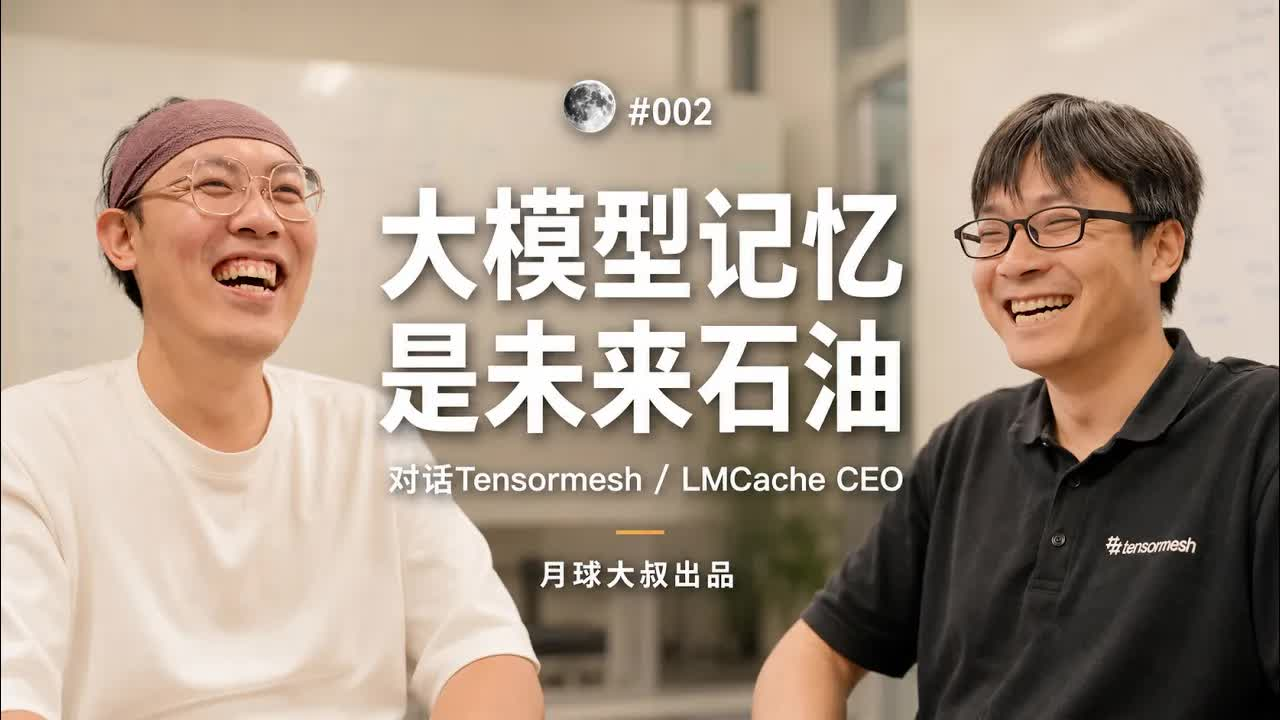
\includegraphics[width=.86\linewidth,height=.27\textheight,keepaspectratio]{cover.jpg}
\par\vspace{6mm}{\small 原节目：江鋆晨: KV Cache，大模型记忆，清华姚班，CMU，教授，开源，视频流媒体\par}
\vspace{4mm}主播：月球大叔\par
{\small 江鋆晨\par}
\vfill 发布：2026-06-09\par
整理：2026-10-25\quad 正文：Gemini Argon\quad 配图与编校：Codex\par
\vspace{4mm}\url{https://www.youtube.com/watch?v=yWTVEG9UIHo}
\end{titlepage}
\begingroup\small\setlength{\parskip}{0pt}\tableofcontents\endgroup\clearpage
\section*{导读}\addcontentsline{toc}{section}{导读}
为什么今天的大语言模型在读完一份十万字代码库后，五分钟后再问一个新问题，往往还要把相同的内容重新算一遍？这不仅是算力账单上的损耗，也是一个典型的计算机系统问题。本讲义根据芝加哥大学计算机系教授、Tensormesh 联合创始人兼 CEO 江鋆晨的深度访谈整理而成。我们将沿着他从清华姚班、卡内基梅隆大学（CMU）流媒体系统研究，一路走到开源项目 LMCache 与大模型基础设施创业的脉络，一步步拆解 KV 缓存（KV Cache）的技术机制。你将读到：前人如何在互联网与流媒体的野蛮生长中提炼出内容分发网络（CDN）等数据层规律；大模型推理中的预填充（Prefill）与解码（Decode）如何分工；CacheGen、CacheBlend 与 LMCache 如何解决大张量传输与非前缀复用难题；以及在智能体（Agent）时代，管理模型运行期内部状态为何会成为修改权重与组织提示词之外的第三条演进路径。
\needspace{8\baselineskip}\section{第一章 兴趣、导师与发现问题的能力}
许多同学初入科研时，习惯等待一个现成的题目去攻克。本章跟随江鋆晨从清华本科到卡内基梅隆大学（CMU，Carnegie Mellon University）读博、再到芝加哥大学任教的经历，探讨研究者如何通过具体的课题尝试辨认个人兴趣，如何在不同风格的导师支持下成长，并逐步建立从技术史和工业一线发现新问题的能力。
\needspace{6\baselineskip}\subsection{从姚班出发，找到自己想解决的问题}
本科生进入科研的起点，往往不是一开始就规划好宏大的学术蓝图，而是在真实尝试中看清自己关心什么。江鋆晨在 2006 年通过数学竞赛保送，2007 年进入清华大学数理基科班，随后考入由姚期智先生创办的计算机科学实验班（简称“姚班”）。据他回忆（00:03:03–00:07:31），当年姚班选拔笔试和面试都集中在数学竞赛题，因此班里既有编程基础深厚的同学，也有像他这样数学突出但计算机背景尚浅的学生。课程设置兼顾理论与编程，早期负责管理学生科研的老师多有理论计算机背景，自然希望学生多尝试理论方向。

真正的兴趣分流发生在第一次做具体课题的时候。大一、大二期间，江鋆晨去了一个网络研究组，接手了一个提升算法性能的问题。他把运行速度提高了不少（具体倍数已记不清），觉得是个不错的突破，便拿去请教姚班一位做理论的老师。老师看完后的第一反应是：既然有了性能提升，能不能进一步证明在特定条件下，这个提升的理论上限就是这么多？这次对话让他意识到两种不同的研究取向：理论研究除了设计新算法，也非常看重对问题深度的理解，常通过证明“不可能性（impossibility）”或严格的性能上限来界定问题的边界；而他自己更关心系统能不能继续突破、性能能不能进一步提高。这里体现的是理论分析与系统工程改进两种不同的学术兴趣，而非学科本身的高下。

有了这次自我认识，他在寻找长期科研方向时更加注重直觉与动手体验。当时系里支持本科生找导师做科研，他和几个室友互不相识系里的老师，就直接按计算机系网页上的字母顺序挨个打电话。前两位老师没接或在出差，第三位接电话的是网络组的刘斌老师。刘斌老师当时虽然也在外地，但非常热情地把他们介绍给组里的博士生唐毅。唐毅尽管自己科研压力不小，却极其耐心地带着这群本科生找课题、读论文、写论文，前后带了三年。宽松纯粹的实验室氛围，让江鋆晨体会到了泡在博士生堆里做研究的乐趣，而不必背负必须按指标发论文的焦虑。

这种按个人节奏探索的心态，也体现在他对大学评价体系的选择上。在同侪压力很大的环境里，不少同学会去竞争清华大学特等奖学金（简称“特奖”）或追求平均学分绩点（GPA）第一。江鋆晨则调侃自己从上海中学数学班到清华姚班都处于“中游”，他更愿意和自己较劲，把精力花在自己真正感兴趣的事情上，甚至连特奖答辩会都不愿去当观众。这种尽量把注意力从单一外部排名转向具体科研问题的处事方式，让他得以在本科阶段轻松投入实验室探索。

\needspace{6\baselineskip}\subsection{导师如何支持不同的学生}
当研究方向从本科延伸到攻读博士学位（PhD）时，行业演进阶段和个人偏好共同影响了课题的选择。2011 年江鋆晨本科毕业申请博士时，在他所接触的领域里，人工智能（AI）和深度学习还不是大家普遍追逐的热点。他回忆大四去自然语言处理（NLP，研究计算机理解与生成人类语言的技术）实验室时，听到的讨论还以支持向量机（SVM）和模式匹配等统计方法为主，深度学习只是组里博士生出去开会听来的新名词；在他当时的观察里，2000 年前后的互联网热潮已过，2010 至 2015 年间行业更关注大数据和云计算，直到 2016 至 2017 年前后计算机视觉等 AI 应用才开始在他身边大规模兴起。与此同时，他在清华网络组虽然做得开心，但课题主要涉及网络安全与隐私。他个人觉得那类安全课题常常侧重于设置限制并严谨证明系统在特定条件下不出安全问题，这与他喜欢突破性能限制的性格不太契合，因此他在申请 CMU 时决定转向更偏向系统性能与架构的网络方向。

在 CMU 选导师的经历（00:16:21–00:22:14），展示了优秀导师支持学生的不同方式。受学长建议，他联系了当时已在硅谷创办视频网络公司的张辉老师，并受邀前往加州面谈。整场会面中，张辉没有灌输自己的课题，而是让江鋆晨站在会议室白板前，痛快地讲自己想做什么。虽然本科生当时的设想在资深学者眼里未必可行，但张辉通过倾听准确捕捉到了这个学生的性格与动力所在。江鋆晨总结自己遇到的两位导师各有千秋：清华的刘斌老师是把纯粹的学术热情和自由度交给学生；CMU 的张辉老师则擅长因材施教，哪怕不直接紧盯每一个执行细节，也能把大方向拆解成学生真心喜欢、愿意主动投入热情的具体课题。

读博期间，江鋆晨还与张辉早年的开门弟子、加州大学伯克利分校教授Ion Stoica展开了紧密合作。Ion Stoica在组里扮演了类似联合导师（co-advisor）的角色，展现出了另一种关键的学术领导力：在同时推进多个项目时，他不仅能理清项目群之间的脉络，还能帮每个学生盯准最核心的目标。江鋆晨用了一个生动的比喻：学生做探索时，往往像在草坪上低头看哪里的草有意思就往哪走；而Ion总能及时让学生抬起头，看清远处那棵作为最终目标的“树”在哪里。

更进一步看，Ion Stoica 之所以能在点对点传输（P2P）、大数据（如分布式计算系统 Spark 与集群资源调度系统 Mesos）以及后来的 AI 服务系统等多个时期都做出有影响力的工作，按江鋆晨的观察，是因为他习惯思考未来五年最重要的技术问题是什么。一旦想清楚下一个五年的核心方向，即使手头原有的路由器服务质量（QoS，保障网络传输延迟与带宽等指标的机制）或 P2P 研究正处于学术发表的高潮期，他也能果断停掉旧方向，把精力集中投向新领域。这种不被既有论文产出束缚、始终对准下一个五年核心问题的视野，给江鋆晨留下了很深的印象。

\needspace{6\baselineskip}\subsection{从解决问题转向提出问题}
博士毕业并完成阶段性过渡后，江鋆晨来到芝加哥大学担任计算机系教授。在北美学术界，从博士生转变为博士生导师（博导），往往会遇到一个角色转换的难关。做学生时，核心任务是“解决问题”，越优秀的博士生通常越是解决具体技术难题的高手；但成为博导后，核心职责变成了“提出问题”或引导别人提出问题。如果老师自己按捺不住动手的热情，既提问题又把问题全解决了，学生就失去了成长的空间。这就像工业界里优秀的程序员被提拔为工程管理者后，需要克制直接替下属写代码的冲动，去学习一套引导团队的新技能。

那么，在顶尖高校做教授最大的优势是什么？江鋆晨认为，除了发表论文、申请基金和培养学生之外，好学校赋予教职人员一种难得的自由——你有机会去研究那些当下别人还不觉得重要、但未来可能改变行业认知的问题。当学生提出一个看起来不合常规的想法时，导师的第一反应可能是怀疑，但如果仔细推敲后发现它有机会改变工业界或学术界对某类系统的既有看法，导师就可以支持学生沿着这条路走下去，把冷门想法做出真正的行业影响力。

在招收和指导博士生时，这种对原创问题的追求也转化为具体的选人偏好。江鋆晨发现，组里最终做出超出预期成果的学生个性各异：有人工程实现强，有人擅长逻辑推演，有人擅长论文写作，也有人对外沟通出色。面对不同性格的学生，导师每次开会都要琢磨合适的沟通方式。而在背景特征上，他个人很看重有过学科竞赛经历的学生，例如后来与他联合创业的坤泰（Kuntai Du）和益华（Yihua Cheng），分别有过化学竞赛和计算机竞赛背景。按他个人的带学生体会，这类有过竞赛经历的学生往往习惯跳跃性的、不完全连续的思维方式，并且乐于尝试别人想不到的突破，这种特质与他自己探索性强的系统研究风格颇为契合。

\needspace{6\baselineskip}\subsection{用研究史辨认下一次变化}
既然提出好问题是研究者的核心能力，那么怎样判断哪些问题在未来会变得重要？江鋆晨在访谈中（00:58:19–01:02:34）分享了两条他自己常用的路径：第一条路径是通过学习技术史和科学史，从历史的演化与相似背景中辨认宏观问题；第二条路径则是与工业界一线保持紧密接触，在工程演进的前沿捕捉刚刚浮现的变化趋势（即数学上象征变化率与增量的 gradient 或 Delta）。

围绕第一条路径，他给研究生和高年级本科生提出了一个实用的学习建议：把博士阶段的高阶专业课（Advanced courses，如高阶操作系统、高阶计算机网络、高阶数据库等）当成“历史课”来上。许多同学读 20 年前的经典论文时，容易觉得里面的具体技术已经过时，甚至嘀咕“怎么几十年前就有人提过类似的想法”。但在学习层面，经典论文的重要价值在于还原当时的历史条件——看前辈研究者在算力、网络带宽或应用规模发生变化时，为什么认为某个问题至关重要，又是如何建立新抽象的。同样，去了解施乐帕洛阿尔托研究中心（PARC，早期研发出以太网与图形用户界面的实验室）或贝尔实验室（Bell Labs）的历史，也能帮助研究者培养对技术演进脉络的敏感度。

当研究者的脑海里有了这些技术史的坐标，面对新现象时就更容易产生跨时代的联想。正如后文第三章将展开的那样，当互联网从静态网页走向视频流媒体、再到今天的大语言模型（LLM）普及，底层基础设施往往会在应用规模扩张的节点上面临相似的数据传输与存储挑战。江鋆晨自己在芝加哥大学讲授高阶课程时，就会梳理技术演进脉络，引导学生思考：既然历史上因为某种应用规模的变化催生了那一代系统，那么今天的技术条件下，下一次结构性的变化可能出现在哪里？将这种历史视角与一线工程观察结合起来，是帮助研究者跳出跟风发论文、寻找长期课题的有效方式。

\begin{knowledgebox}{理论边界分析与系统工程突破的互补性}
在计算机科学中，理论研究与系统研究往往关注同一个问题的不同侧面。理论计算机科学既设计高效的新算法，也常寻求普适的数学规律——例如通过复杂度分析或下界证明，界定算法在给定约束下难以逾越的性能上限（Impossibility Results），从而 clarify 问题的数学边界。系统与工程研究则更关注在真实硬件、真实网络负载和特定应用分布下，如何通过架构重组、协议优化或启发式设计不断突破现有系统的性能瓶颈。理解两者的侧重，有助于本科生在早期科研尝试中看清自己更喜欢严谨的形式化推演，还是更喜欢在真实系统中持续改进工程性能。
\end{knowledgebox}
\begin{importantbox}{如何把高阶系统课（Advanced Courses）读成技术史}
阅读十年前甚至二十年前的计算机系统经典论文时，不应只看当时的实验数据或具体代码实现（这些往往已随硬件换代而过时），而应重点提取三个历史维度：第一，时代约束，即作者写论文时硬件、网络或应用规模刚发生了什么突变；第二，问题定义，作者如何把工业界杂乱的痛点抽象成一个清晰的科学问题；第三，演化脉络，这篇工作启发了后续哪些工业标准，又因为什么新条件的出现而被后来的架构取代。用这种方式读论文，积累的是识别“下一代真问题”的判断力。
\end{importantbox}
\begin{table}[H]\centering\small
\caption{科研成长阶段的三种引导模式与角色转型}
\begin{tabular}{>{\raggedright\arraybackslash}p{\dimexpr(\linewidth-6\tabcolsep)/3\relax}>{\raggedright\arraybackslash}p{\dimexpr(\linewidth-6\tabcolsep)/3\relax}>{\raggedright\arraybackslash}p{\dimexpr(\linewidth-6\tabcolsep)/3\relax}}
\toprule
人物或阶段 & 核心引导方式与关注点 & 对学生与研究工作的实际作用\\\midrule
刘斌老师与唐毅学长（本科科研启蒙） & 提供宽松纯粹的探索环境，由高年级博士生手把手带读论文与入门课题 & 消除本科生对发表指标的焦虑，在动手实践中发现对网络系统性能突破的真实兴趣\\[4pt]
张辉老师（CMU博士阶段） & 先倾听学生的想法与性格偏好，因材施教地将大方向转化为学生感兴趣的课题 & 让研究者产生内驱力，把个人突破极限的偏好与流媒体等前沿产业需求结合起来\\[4pt]
Ion Stoica教授（跨项目合作） & 在多个并行项目中理清全局脉络，帮低头探索的学生看清远处的“目标之树”，果断切换五年周期的新方向 & 防止研究陷入局部细节，示范如何根据未来五年的核心价值重构研究版图\\[4pt]
从博士生到博导的转型（芝加哥大学任教） & 克制替学生直接解决具体难题的冲动，转向提出问题、评估长期价值并激发不同特质的学生 & 利用高校的学术自由度，探索当下尚未形成共识但未来可能改变行业认知的研究方向\\[4pt]
\bottomrule\end{tabular}\end{table}
当研究者从解决具体技术难题的博士生转型为需要提出问题的独立学者时，究竟该依靠什么线索去判断哪些新问题值得投入？下面的机制示意图将本章讨论的两条核心路径汇总到了同一个判断框架中。
\begin{figure}[H]\centering
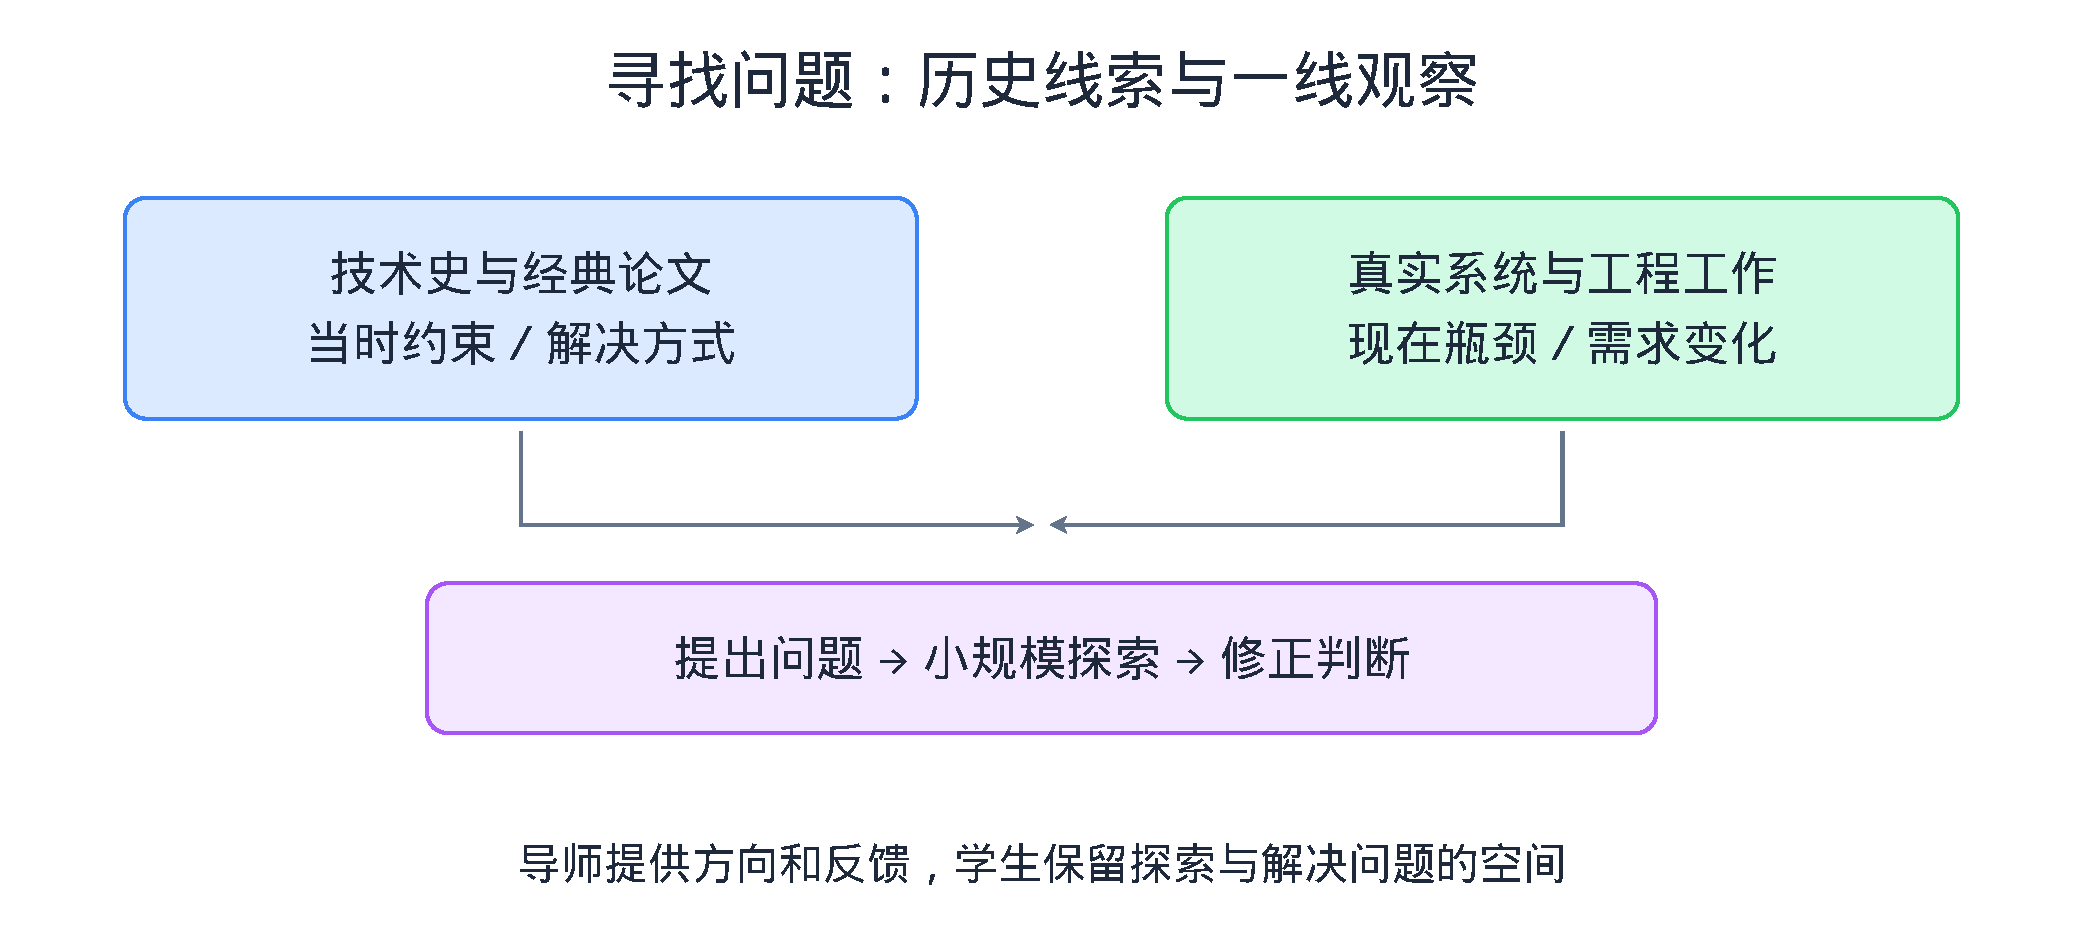
\includegraphics[width=\linewidth,height=.68\textheight,keepaspectratio]{assets/question-discovery.pdf}
\caption{寻找问题：历史线索与一线观察；依据节目口述整理（00:54:35–01:02:16）}
\end{figure}
\begin{knowledgebox}{读图：第一章 兴趣、导师与发现问题的能力}
图上方左右并列两个输入方框：左侧为“技术史与经典论文：当时约束／解决方式”，右侧为“真实系统与工程工作：现在瓶颈／需求变化”。两股线索通过向下的折线箭头汇聚到下方的核心长框“提出问题 \ensuremath{\rightarrow} 小规模探索 \ensuremath{\rightarrow} 修正判断”。图底部文字点明了协作关系：“导师提供方向和反馈，学生保留探索与解决问题的空间”。
\end{knowledgebox}
这种将历史纵深与一线增量结合的探索闭环，不仅解释了江鋆晨在高校带学生的思路，也将在下一章他深入视频流媒体与播放器工程的经历中得到具体印证。
\needspace{6\baselineskip}\subsection{本章小结}
\begin{enumerate}
\item 科研兴趣需要在具体课题尝试中辨认：通过对比理论上限证明与系统性能改进，江鋆晨明确了自己突破工程极限的研究偏好。
\item 优秀的学术指导各有侧重：从宽松自由的启蒙、因材施教的课题匹配，到看清全局目标并果断切换五年研究方向，不同导师帮助学生建立起完整的学术视野。
\item 独立研究者的核心能力是提出好问题：无论是从博士生转型为博导，还是判断未来趋势，都需要结合对技术史（高阶课程经典论文）的深度理解与对工业界一线变化的敏锐观察。
\end{enumerate}
\needspace{8\baselineskip}\section{第二章 流媒体如何教会我们理解基础设施}
今天我们在手机和电脑上随时观看高清视频，早已习以为常，但在 2010 年前后，大规模互联网视频才刚刚迈过产业拐点。本章顺着江鋆晨在读博与工业界实习期间研究视频流媒体的经历，探讨一项应用普及后如何倒逼底层基础设施（Infrastructure，简称 Infra）演进，以及研究者如何深入工程一线发现共性约束，并从中提炼出跨越时代的“数据层”思路。
\needspace{6\baselineskip}\subsection{HTTP 和宽带让视频分发走向普及}
在 2010 年以前，通过互联网向大众流畅传输长视频或高清直播是一件门槛很高的事。江鋆晨回忆（00:26:18–00:30:26），2008 年北京奥运会做网络直播时，还需要联合多家公司专门搭建一套定制系统；当时的视频网站中虽然 YouTube 很火，但整个线上视频流媒体（Video Streaming，指边传输边播放的音视频技术）行业远未成熟。转折点出现在 2010 年前后：一方面北美等地区的家庭宽带普及率大幅提升，另一方面 Netflix、HBO、BBC 等媒体与内容公司意识到，可以直接通过互联网把视频传给用户。一时间，各家媒体公司都在制定自己的流媒体战略，其迫切程度就像今天许多企业都在制定 AI 战略一样。

然而，当媒体公司急需大规模上线视频产品时，虽然此前已有专用流媒体协议探索，但业界还没有一套现成的、经过全网普及验证的统一视频分发系统。当时的互联网基础设施主要是围绕网页浏览广泛部署的，核心是超文本传输协议（HTTP，浏览器与服务器之间广泛使用的应用层传输协议）。此前不少人认为围绕网页设计的 HTTP 未必适合传输连续的视频流，但媒体公司为了尽快触达用户，最现实的选择就是复用 HTTP——因为它是当时各类网络运营商和防火墙普遍默认放行、部署最广的协议。当高带宽用户群遇上基于 HTTP 的分块视频传输，这条依托现有基础设施的技术路线很快跑通了。

一旦商业和技术可行性得到验证，工业界便进入了快速扩张的“野蛮生长”阶段。苹果、亚马逊、谷歌等公司纷纷基于网页传输格式各自搭建视频系统。一线工程团队的首要任务是让产品尽快上线运行，往往无暇从全局去梳理这些仓促上马的协议会对整个互联网造成什么影响，也还来不及系统研究什么样的抽象和算法能让系统更可持续、下一代架构又该如何演进。这种“产业界已经在高频使用、但尚缺系统性设计原则”的阶段，恰好为学术界提供了丰富的研究课题。

站在最终用户的角度，视频流媒体的目标听起来非常简单：画面清晰度（分辨率）要高，播放要流畅、不能频繁卡顿。但要实现这个朴素的目标，单靠提高某一段网络的带宽远远不够。从学习的角度拆解，一条完整的视频链路涵盖了源端服务器、视频编解码（将原始画面压缩为较小体积的数据流并在终端还原）、传输协议、骨干与接入网络，直到用户手机或电脑上的播放器。这是一套环环相扣的复杂工程，任何一个环节配合不当，用户就会立刻在屏幕上感受到卡顿或画质下降。

\needspace{6\baselineskip}\subsection{从播放器内部发现真实约束}
面对各大公司各自搭建、互不透明的视频系统，研究者该如何迈出第一步？江鋆晨在读博第一年做的第一个印象深刻的项目，就是对主流视频平台的传输机制做反向工程（Reverse Engineering，通过观测外部行为和数据包特征来分析系统内部的设计逻辑）。他连续熬夜几个星期，抓取并分析苹果、亚马逊、谷歌等系统的网络数据包，一点点摸清它们在包里放了什么内容、遵循怎样的控制协议。这段经历让他干劲十足，因为在他的印象里，自己当时属于最早把各家工业系统的真实做法、共同弱点与共性挑战放在一起梳理清楚的研究者之一。

除了在实验室里观测外部数据包，真正帮他看透流媒体系统底层约束的，是一次深入工业界一线的实习（00:47:13–00:53:56）。在担任教职前，江鋆晨共有过四次工业界经历，其中三次在微软研究院（Microsoft Research），一次在导师张辉联合创办的流媒体技术公司 Conviva 做工程产品。他坦言，虽然在微软研究院的实习顺利产出了论文，但对后续学术研究帮助最大的，恰恰是在 Conviva 直接写产品代码、不写论文的那一次。当时张辉交给他的任务是开发视频播放器，并明确叮嘱他：实习期间完全忘掉发论文和做研究的事，专心把产品做出来。

视频播放器属于很底层的客户端工程，许多工程师都觉得棘手，学术界更少有论文直接研究怎么写播放器。江鋆晨当时先用 Adobe 环境下的一套冷门语言编写播放器，后来又用 C 语言开发苹果生态的播放组件。正是这段看似纯粹“写工程代码”的经历，让他成了当时网络视频传输领域的博士生和老师里，少数真正清楚播放器内部运作细节的人：哪些算法优化播放器底层能够支持，哪些优化写进论文里好看但在播放器里无法奏效；哪些工程瓶颈是暂时的、过两年技术升级就能解决，哪些又是不同厂商播放器共同面临的结构性难题。

基于这段实践经验，江鋆晨经常建议自己的学生：如果有机会去工业界做与研究方向相关的实习，不要带着研究者的偏见或“赶紧凑一篇论文”的心态去，而要以纯粹的“工程师心态”融入团队。短短三个月的暑期实习，不足以把一个学生训练成资深的工程专家，却能让你融入一线工程师的日常工作中，亲眼看到他们每天在争论什么、真实系统里什么事情难、什么事情容易。相比之下，学术界有时容易陷入自我循环的气泡（Bubble）——几篇论文互相引用、彼此觉得某个假设的问题重要，研究者却未必见过真实问题长什么样。一线工程师通常不关心发论文，但他们今天在单点工程上遭遇的痛点，等实习生回到学校沉淀思考一年后提炼成论文，过一两年往往就会变成行业里许多团队都会碰到的重要问题。

\needspace{6\baselineskip}\subsection{把播放体验汇集成网络观测}
理解了单个播放器和单条视频流的运作后，江鋆晨与导师张辉、Ion Stoica 以及另一位导师 Vyas Sekar 合作推进了博士期间第二个代表性工作：把全球范围内的视频播放变成一张监测互联网质量的观测网（00:32:41–00:37:39）。这个项目的构思源于一次视角转换：当用户打开手机或电脑看视频时，不仅是在消费内容，视频播放的流畅度与清晰度本身，也反映了从服务器端到用户终端这条网络连接的质量。如果把全球各地大量的视频播放放在同一个维度下看，每一次播放其实都是在对网络局部状态做实时测量。

顺着这个逻辑往下推，既然视频流量如此庞大且分布广泛，能不能用大数据的方法把这些分散的视频质量监测结果汇总起来，辅助分析当前互联网哪里出现了问题、哪里变慢了、哪里需要调配更多带宽？这也正是当时正在推进大数据研究的 Ion Stoica 对该课题感兴趣的原因——它是早期用大数据方法去全局优化互联网级应用的尝试之一。当然，从系统原理来看，单次终端异常有时可以通过单机或局部日志排查，而客户端观察到的卡顿或画质下降受多环节因素影响，单靠播放观测相关性并不能自动定位出唯一的故障节点；但当大量并发的播放数据汇聚在一起时，通过统计关联不同区域与链路的特征，就能帮助发现共性问题并指导优化调度。

然而，提出超前的问题往往意味着要承受审稿周期的煎熬。江鋆晨回忆，这篇用大数据优化网络视频传输的论文前前后后投了五次才最终被接收，前四次全部被拒。为了说明这种探索的风险，他分享了张辉老师在CMU给博士新生做15分钟迎新演讲时的一个故事：张辉让一位美国学生在白板上画三只一模一样的抽象小狗，然后问大家这三只狗有什么区别。学生打趣说某只狗尾巴没画好，张辉却指出：真正的区别在于“只有第一只狗是第一只狗”。

在这个比喻里，跑在最前面的“第一只狗”，看到前面有根骨头有机会第一个吃到；哪怕前面是个坑掉下去了，也替大家探明了风险；而跟在后面的两只狗作为追随者，虽然能看着第一只狗掉坑而绕开走，但若想做出真正领先的研究，就得有做“第一只狗”并承担早期探索风险的意愿。江鋆晨个人觉得，在计算机系统科研中，只要选准了真实的新方向去探索，即便早期投稿碰壁，往往也能在摸索中做出有价值的工作。

\needspace{6\baselineskip}\subsection{从 CDN 到应用的数据层}
无论是反向剖析协议还是做全局质量观测，流媒体研究最终都会指向一个关键基础设施——内容分发网络（CDN，Content Delivery Network，通过在不同区域部署缓存服务器，将内容就近分发给用户的网络架构）。江鋆晨指出（00:38:01–00:46:58），CDN 早在网页（Web）时代就已经诞生，而到了视频流媒体时代又再度兴盛。原因在于，视频数据量远大于普通网页，骨干网与长途传输成了突出的中间瓶颈；CDN 通过结合缓存策略将热门或常访问的视频内容部署到离用户更近的节点，缩短了传输路径。当然，缩短网络路径并不能消除编解码或终端播放器等其他环节的瓶颈，但它大大缓解了视频跨网分发的压力。

如果跳出视频行业往回看，为什么 CDN 在网页时代重要、在流媒体时代重要，甚至在今天依然能看到它的影子？江鋆晨基于技术史形成了一个自己的判断：当某类应用的普及规模足够大、有相当比例的人在高频使用时，系统里往往会演化出一层专门的“数据层（Data Layer）”，用来让核心数据的分发、共享和分析变得更高效。在网页和视频时代，这层能力体现为 CDN；到了大数据时代，底层存储体现为 Hadoop 分布式文件系统（HDFS，负责跨机器存储海量数据的文件系统），并配合其上的分布式计算系统 Spark 实现高效分析；而到了今天的大模型时代，他认为同样会生长出服务于 AI 的数据层——这正是后文将深入探讨的 KV 缓存（KV Cache）管理。

这种对“大规模应用呼唤对应系统层”的思考，也直接影响了江鋆晨博士毕业后的研究转向。在正式前往芝加哥大学任教前，他按照北美学术界常见的做法留出一年过渡期（Gap year），前往微软研究院寻找新方向。当时他已经完成了用数据与 AI 方法优化网络的博士课题，希望转向为 AI 构建系统（System for AI）。在这一领域中，他很早就形成了一个鲜明的个人研究偏好：不做模型训练（Training）系统，而是专注推理（Inference，即用训练好的模型服务实际请求）系统。

为什么在当时不少人关注训练系统时，他选择聚焦推理？在江鋆晨个人看来，模型训练固然重要，但一个模型训练完成后会被长期反复调用，其完整生命周期中绝大部分运行时间都花在推理和服务用户上；一旦应用场景大规模铺开，推理就会成为长期存在的系统瓶颈。虽然当时推荐、语音等领域已有 AI 推理应用，但在他关注的系统方向上，计算机视觉与视频分析（Video Analytics）既初具规模，又与他此前积累的视频系统经验天然契合，于是他在微软研究院和芝加哥大学任教初期便从视频分析系统切入。这段经历也为几年后大语言模型爆发时迅速切入推理缓存管理埋下了伏笔。

\begin{warningbox}{端到端流媒体链路中的多环节约束与观测边界}
初学者常以为视频卡顿单纯是因为“网速慢”，或者以为只要接入内容分发网络（CDN）就能解决所有播放问题。实际上，流媒体是一条端到端的复杂系统链路：首先，CDN 的作用是按策略将内容缓存在离用户较近的节点以缓解长途传输瓶颈，但它无法消除最后一公里接入网（如拥挤的 Wi-Fi 或蜂窝网络）的波动；其次，即使网络传输正常，如果源端服务器调度过载、编解码参数与码率自适应算法不匹配，或者终端视频播放器内部缓冲与解码管理存在缺陷，用户依然会遇到画面卡顿或清晰度下降。同理，单机问题虽可借助本地日志排查，但当汇集全网播放指标做大数据分析时，统计相关性主要用于识别区域拥塞与共性瓶颈，而非直接替代单点硬件故障诊断。
\end{warningbox}
\begin{importantbox}{如何在工业界实习中运用“工程师心态”发现研究问题}
博士生去工业界实习时，容易走入两个极端：要么去做与自身研究方向毫无关联的日常杂活；要么带着强烈的学术预设，一进公司就急着找能发论文的现成切入点。江鋆晨提倡的“工程师心态”，是指在与研究领域相关的工程实习中，暂时放下写论文的执念，作为产品团队的一员去写底层代码、参与日常工程讨论。三个月的时间虽不足以把人变成资深工程专家，却能让你看清真实系统的硬约束——哪些优化在现有架构里跑不通，哪些痛点是一线工程师天天面对却还没人写论文总结的。等实习结束回到学校，再切换回研究者视角把这些观察提炼成科学问题，往往能找准极具潜力的研究方向。
\end{importantbox}
\begin{table}[H]\centering\small
\caption{不同技术时代的大规模应用与对应的数据层（Data Layer）演进}
\begin{tabular}{>{\raggedright\arraybackslash}p{\dimexpr(\linewidth-6\tabcolsep)/3\relax}>{\raggedright\arraybackslash}p{\dimexpr(\linewidth-6\tabcolsep)/3\relax}>{\raggedright\arraybackslash}p{\dimexpr(\linewidth-6\tabcolsep)/3\relax}}
\toprule
技术阶段与核心应用 & 面临的数据与传输瓶颈 & 数据层机制与系统实践关系\\\midrule
网页与流媒体时代（Web \& Video Streaming） & 宽带普及后海量用户并发请求网页与高清视频，跨网远距离传输延迟高、骨干网带宽承压 & 通过内容分发网络（CDN）将静态网页与视频切片缓存至离用户更近的边缘节点，并配合基于HTTP的自适应传输与终端播放器优化保障流畅体验\\[4pt]
流媒体全局质量监测（大规模网络应用优化） & 各地区网络状态动态变化，单点探测难以覆盖全球真实用户的连接质量与异常分布 & 将全球数以千万计的视频播放会话视为分布式网络探针，利用大数据（Big Data）汇总播放质量指标，统计推断网络拥塞区域并指导流量调度\\[4pt]
大数据时代（企业与互联网数据分析） & 海量日志与业务数据超出单机存储与处理上限，跨节点数据读写与分析效率成为瓶颈 & 以Hadoop分布式文件系统（HDFS）作为底层分布式存储数据层，配合Spark等分布式计算引擎实现高效的数据共享与并行分析\\[4pt]
大模型推理时代（LLM Inference \& Agent） & 高频多轮交互与长上下文处理产生庞大的注意力中间状态，重复计算消耗大量算力与等待时间 & 将模型内部生成的KV缓存（KV Cache）作为新型核心数据，构建解耦的缓存存储与传输层，实现跨请求与跨实例的高效复用\\[4pt]
\bottomrule\end{tabular}\end{table}
用户在屏幕上感知的清晰度与流畅度，并不是某一段网络带宽单独决定的，而是端到端复杂工程协同的结果；反过来，海量的终端播放体验也能汇集成观测网络状态的窗口。下图展示了这一正向传输与反向观测的闭环。
\begin{figure}[H]\centering
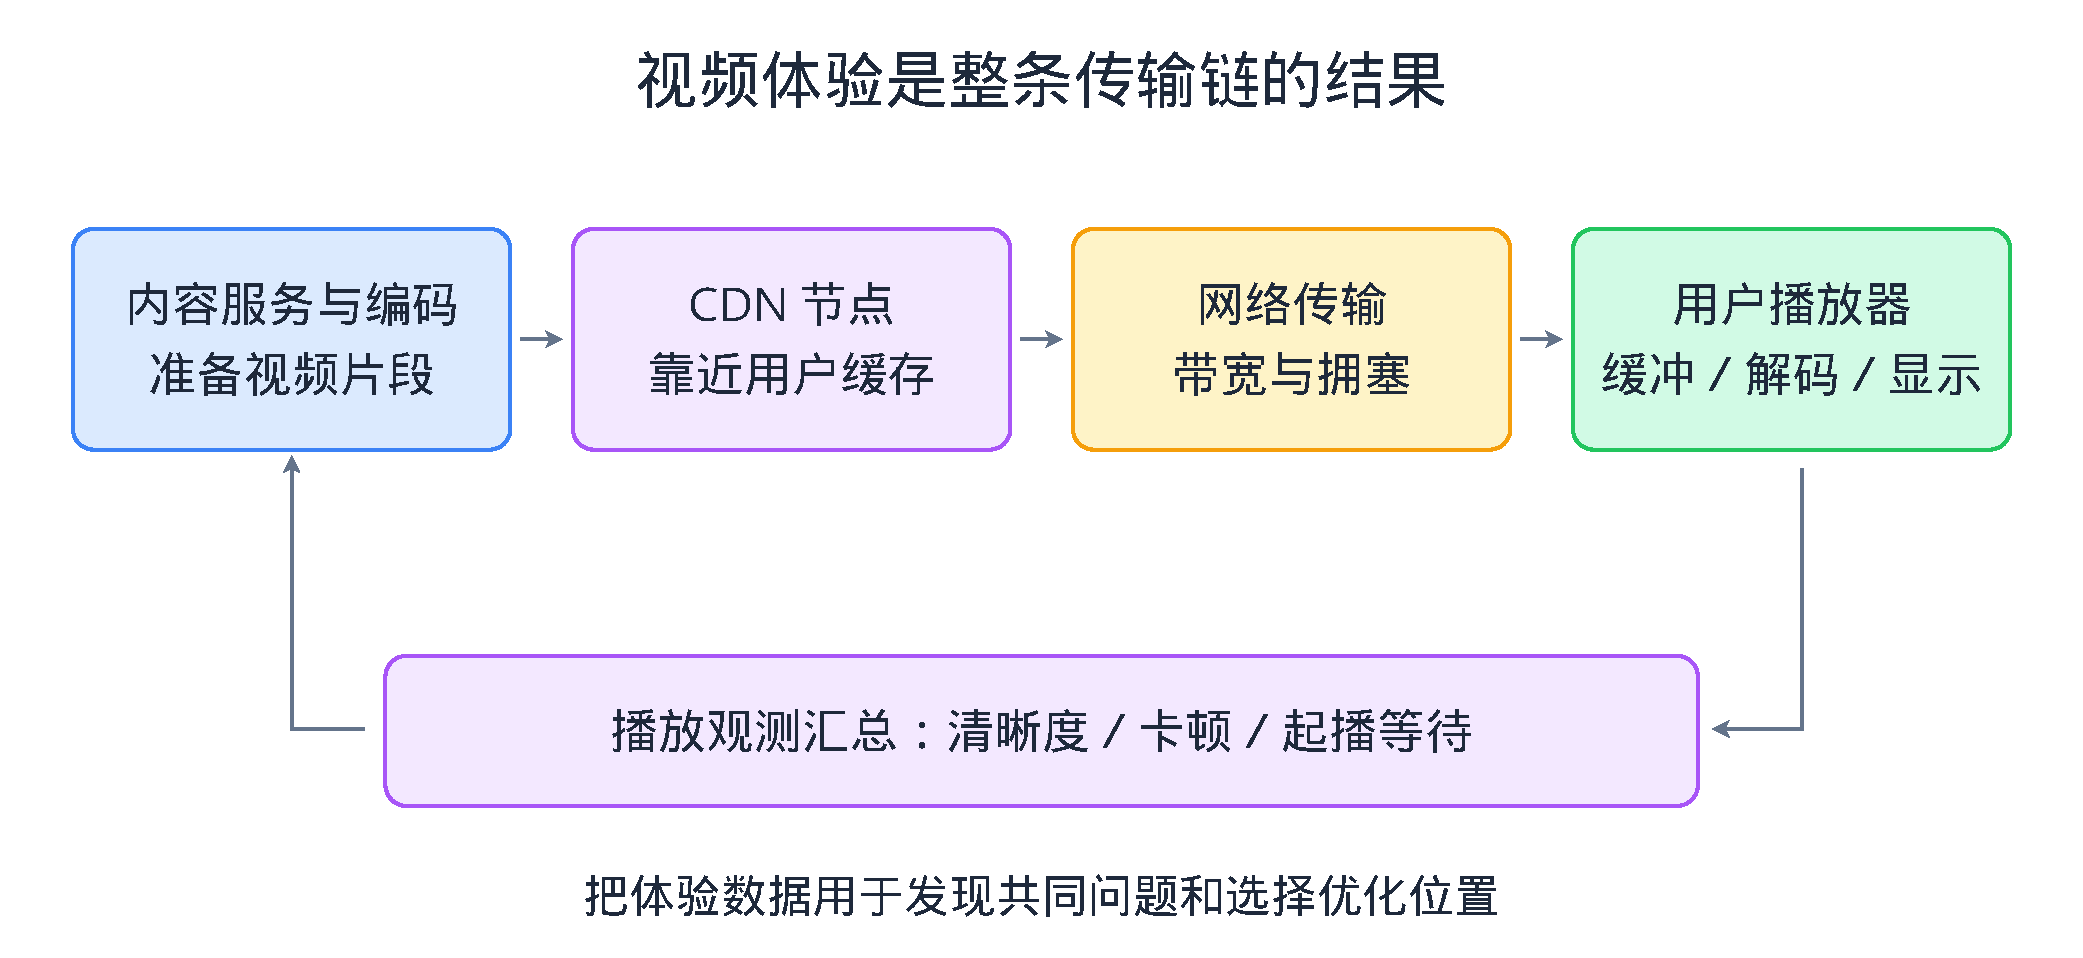
\includegraphics[width=\linewidth,height=.68\textheight,keepaspectratio]{assets/streaming-observation.pdf}
\caption{视频体验是整条传输链的结果；依据节目口述整理（00:26:18–00:39:54；00:47:13–00:53:56）}
\end{figure}
\begin{knowledgebox}{读图：第二章 流媒体如何教会我们理解基础设施}
图上行从左到右由四个方框经箭头依次相连：“内容服务与编码：准备视频片段”指向“CDN 节点：靠近用户缓存”，再指向“网络传输：带宽与拥塞”，最终到达右侧的“用户播放器：缓冲／解码／显示”。从右侧“用户播放器”引出一条向下再向左的箭头，汇入下方的宽框“播放观测汇总：清晰度／卡顿／起播等待”，并由左端箭头反馈回最左侧的“内容服务与编码”。底部总结为“把体验数据用于发现共同问题和选择优化位置”。
\end{knowledgebox}
从终端播放器约束到全网质量汇总，流媒体时代围绕“就近缓存与全局调度”建立起的数据层思维，为下一章理解大模型推理中的中间状态缓存提供了直观的历史参照。
\needspace{6\baselineskip}\subsection{本章小结}
\begin{enumerate}
\item 产业拐点常始于既有基础设施上的快速扩张：2010 年前后宽带普及与通用 HTTP 传输的结合推动了视频流媒体普及，各家公司各自搭建系统，为学术界留下了提炼共性问题与系统抽象的空间。
\item 深入工程底层有助于看清真实约束：无论是通过反向工程分析各家数据包，还是以“工程师心态”在 Conviva 编写视频播放器，一线工程体验能帮助研究者避开学术气泡，敢于承担探索风险去做探路的“第一只狗”。
\item 大规模高频应用往往需要高效的数据层：从流媒体时代的 CDN、大数据时代的 HDFS 到大模型时代的 KV Cache，理解数据分发与共享的历史脉络，并聚焦占模型运行周期大头的推理环节，是跨时代迁移系统研究能力的重要线索。
\end{enumerate}
\needspace{8\baselineskip}\section{第三章 大模型为什么需要缓存自己的计算}
从流媒体网络转向大语言模型基础设施，看似跨度很大，实则沿着同一条系统演进线索：当一项应用走向高频普及，系统底层往往需要专门的数据层来承接核心数据的传输与复用。本章沿着江鋆晨团队在 2023 年初的研究转向，解析大模型推理中预填充（Prefill）与解码（Decode）的计算分工、KV 缓存（KV Cache）的张量生成机制与体积估算，以及保存中间计算状态如何影响算力与存储的权衡。
\needspace{6\baselineskip}\subsection{ChatGPT 的变化先发生在使用广度}
在 2023 年初之前，江鋆晨的课题组主要研究视频网络与计算机视觉类的 AI 系统，并未做过大语言模型。转机发生在 ChatGPT 发布一两个月后（01:06:17–01:13:46）：当时网上的讨论铺天盖地，实验室里的学生——包括学生 Yuhan（Yuhan Liu）和坤泰（Kuntai Du）等最早推动此事的成员——几乎每天都在追问导师能不能做点与 GPT 相关的课题，甚至连当年 1 月份计算机网络顶会 SIGCOMM 的论文截稿日（Deadline）都提不起劲去赶了。面对学生的热情，当时学术界不少老师的第一反应是谨慎的，觉得这可能只是一个流行词（Buzzword）或单一公司的应用热潮（Hype），系统研究者不必为了一个应用轻易改变研究方向。

江鋆晨最初也有类似的顾虑，但在被学生们反复推动着深入讨论了几次后，他的看法发生了转变。打动他的并不是 ChatGPT 当时的回答质量有多高——事实上，当时一些早期代码辅助工具写出的代码还很难直接用，底层 Transformer 架构也已经问世多年；真正让他感到不同的是 AI 的“使用广度”与大众兴趣。在此之前，无论是语音分析还是计算机视觉，AI 大多是特定场景下的零散功能；而 ChatGPT 刚出来一两个月，他去餐馆吃饭时都能听到邻桌看似做保险等各行各业的普通人在热烈讨论。在他看来，这是第一次有一个 AI 产品展现出让各行各业的人在日常都想去使用的潜力。

对于做计算机网络与系统出身的人来说，这种广泛的普及兴趣是一个熟悉的历史信号。江鋆晨在当时将其判断为 AI 领域的“互联网时刻（Internet Moment）”：就像 20 世纪 90 年代末至 21 世纪初人们意识到所有计算机可以互联、大家都想上网一样，或者像早期个人电脑（PC）刚问世时虽然实际功能还没宣传得那么全，却彻底激发了大众的想象力一样。一旦用户想用、爱用的正循环飞轮转起来，底层基础设施（Infra）就会迎来大量的优化需求。

基于这一历史类比，江鋆晨对课题组做出了一个果断的决定：让学生们把已有的收尾论文写完以保证毕业，同时支持想做新方向的学生全面转向大语言模型推理优化，哪怕当时距离他评终身教职（Tenure）只有两年、甚至要承担一年发不出新论文的风险。那么，网络系统背景的团队该从大模型的哪个具体问题切入？网络与系统研究擅长处理体积庞大的数据流，而纯文本提示词（Prompt）本身的字节数很小；当时多模态视频生成又还太慢、不够成熟。一番排查后，他们发现模型内部在运行过程中生成的 KV 缓存（KV Cache）不仅体积庞大，而且可以保存、传输与跨请求复用，正好契合了网络与系统研究者的技术特长。

\needspace{6\baselineskip}\subsection{Prefill 和 Decode 做了不同的工作}
要理解为什么大模型内部会产生庞大的缓存数据，首先需要拆解大模型推理的两个主要阶段（01:31:14–01:34:37）：预填充（Prefill）与解码（Decode）。在学习大模型系统时，可以把一次完整的请求响应类比为“先阅读理解、后逐字输出”的过程：当用户输入一段长文本或参考资料时，模型首先要处理整段输入词元（Token，模型切分和处理文本的基本单位），建立对上下文的理解并算出每一层的中间状态，这个输入分析阶段就叫 Prefill；一旦输入理解完成，模型便进入 Decode 阶段，一个 Token 接一个 Token 地顺序生成回答。

在日常使用中，人类用户的直观感受很容易产生一个偏差：大家盯着屏幕等待模型一个字一个字地往外蹦，感官上觉得绝大部分等待时间都在生成输出（Decode），因而容易以为输出阶段就是算力消耗的全部重点。市面上不少新型推理芯片也将硬件创新重心放在加速 Decode 阶段、提升每秒生成的 Token 数量上。加快输出速度确实非常关键，因为它直接决定了用户肉眼感知的生成快慢与交互体验。

不过，江鋆晨提醒，如果切换到基础设施的算力分配视角，在长上下文与智能体（Agent，能通过多轮交互调用工具、与环境互动以完成复杂任务的 AI 系统）等工作负载下，耗费 GPU 算力的重头往往在处理输入的 Prefill 阶段。他的分析来自智能体工作负载的特征：在智能体的运行轨迹（Trace）中，单次生成的输出通常只有几千到上万个 Token，而输入的上下文却动辄达到几十万甚至上百万个 Token——因为历史对话、之前生成的输出以及调用工具返回的结果，往往会不断累积或筛选进入后续轮次的输入中。

这种“长输入、短输出”的不对称性，使得GPU在Prefill阶段承受了极高的并行计算压力。用户只关心屏幕上的字蹦得快不快，却看不见后台为了“读懂”几十万字的背景资料所付出的巨额算力成本。因此，专门针对Decode加速的硬件创新与针对Prefill阶段的软件缓存优化非但不是互相替代的冲突关系，反而是从输出与输入两端互补配合的系统工程。

\needspace{6\baselineskip}\subsection{K、V 张量如何保存已算过的上下文}
为什么 Prefill 阶段算完的结果可以被保存下来？这要回到自回归 Transformer 架构中的因果自注意力机制（Causal Self-Attention，模型在每一层通过计算当前词元与前序词元的相关性来捕捉上下文语义的机制）。作为基础机制解释，当模型在每一层处理输入 Token 时，会通过线性变换为每个 Token 生成三个向量：查询（Query，简称 Q）、键（Key，简称 K）和值（Value，简称 V）。在固定模型权重、相同前序序列与兼容位置配置的因果自注意力下，排在后面的 Token 不会反过来改变前面已处理 Token 的表征；后续生成新 Token 时，只需要用当前 Token 的 Q 去和前面历史 Token 的 K、V 做注意力计算。为了避免每生成一个新词都把前面的文本从头算一遍，系统会把算好的 K 和 V 张量（Tensor，多维数组结构的数据）暂存在显存里，这就是 KV Cache。

为了通俗说明 KV Cache 在模型中的角色，江鋆晨打了一个比方（00:40:08–00:44:25）：如果把线性排列的原始文本比作一本小说，把 KV Cache 比作拍出来的电影，人类看电影往往比读文字更直观高效；类似地，原始文本是给人读的，而 KV Cache 就像是“给大模型看的视频”。它是模型在运行过程中自己生成的内部记忆状态——人类肉眼看过去只是一堆浮点数矩阵，但生成它的同源模型一旦加载这些张量，就能直接恢复出对应上下文的注意力状态，而不必重新做一遍完整的文本预填充（Prefill）计算。

从系统资源开销来看，这段“模型内部状态”的体积相当可观。以常规的自回归 Transformer 推理为例，在批大小（Batch Size）为 1 的教学假设下，保存一段上下文所需的 KV 缓存字节数可以用以下基础公式估算：
\[
\text{KV Cache Bytes} = 2 \times L \times T \times H_{kv} \times D_h \times B
\]

其中，因子 \(2\) 代表 Key 和 Value 两份张量，\(L\) 为模型的 Transformer 层数，\(T\) 为缓存的 Token 数量，\(H_{kv}\) 为每层用于键值计算的注意力头数（KV Heads），\(D_h\) 为每个注意力头的维度（Head Dimension），\(B\) 为每个数值元素占用的字节数（例如半精度浮点数 FP16 或 BF16 占 2 字节，8 位量化占 1 字节；量化通过减少每个元素的位宽来缩小体积）。现代大模型常采用分组查询注意力（GQA，让多个查询头共享同一组键值头以减小 \(H_{kv}\)）或多查询注意力（MQA，所有查询头共享单一键值头），也会结合混合架构、量化或结构裁剪来控制体积；但随着上下文长度 \(T\) 增长到数万乃至数十万 Token，KV Cache 依然会占用数 GB 到数十 GB 的空间（注：张量在代码中的具体维数取决于是否将批大小、层数、KV 头数、序列长度和头维度分别作为独立维度展开）。

需要明确的是，直接做精确前缀复用是有技术前提的。由于 KV 张量的数值取决于模型权重、分词结果以及位置编码（标记词元在序列中先后位置的数学表示），只有在使用相同模型、且新请求的输入包含相同的 Token 前缀与兼容的位置及执行配置时，之前保存的这段前缀 KV Cache 才能直接加载复用，并在此基础上继续处理后续新增的提问 Token（至于前序内容变化后的跨片段复用，将在第四章介绍）。

\needspace{6\baselineskip}\subsection{重复输入何时值得保存与加载}
既然KV Cache体积如此庞大，为什么我们还要费力把它存下来？江鋆晨用程序员辅助编程的场景算了一笔直观的工程账（01:24:21–01:29:42）。假设你把一个庞大的代码库（Program）交给大模型，让它先通读代码再添加一个新功能。在这个请求中，可能90\%以上的输入Token都是这份已有的代码库，用户真正提问的指令只占很小一部分。模型第一次处理时，必须耗费GPU算力把整个代码库做一遍Prefill，生成对应的KV Cache。

如果系统像早期推理引擎那样，在单次回答结束后就把 GPU 显存里的 KV Cache 直接丢弃（Evict），那么五分钟后当你想让模型在同一个代码库上修改另一个功能时，模型就会“忘记”刚才算过的状态，只能把那占输入 90\% 的代码库再从头算一遍。反之，如果把第一次生成的 KV Cache 像保存文件一样存下来，下次遇到包含相同代码库前缀的请求时直接加载（Load）回 GPU，就能跳过这部分占输入 90\% 的重复 Prefill 计算——这就是 Tensormesh 官网提出“不要为重复计算付费”这句标语所对应的典型场景。

当然，把庞大的 KV 张量存下来并重新加载，也会增加对存储系统的需求。在访谈开头（00:01:17–00:02:43）聊到近期存储设备涨价时，主持人开玩笑称做 KV 缓存创业的他们是“罪魁祸首”。江鋆晨对此从市场供需角度谈了自己的看法：他认为存储价格上涨主要是短期供需不平衡导致的，随着上游产能跟上，价格预计会逐步回落；但更值得关注的趋势是——过去大家谈论 AI 往往只盯着 GPU 算力，却容易忽略“算力用得越多，模型运行生成的中间数据（如 KV Cache）也会越多，进而推动对存储容量与带宽的需求同步上升”。

在工程实践中，保存和加载 KV Cache 需要综合权衡“GPU 重算开销”与“存储及传输开销”。当某段上下文前缀被复用的频率较高，且从外部存储介质将 KV Cache 加载回 GPU 的时间快于 GPU 重新计算该段 Prefill 的时间时，缓存复用就能缩短这部分的计算等待，帮助改善首字延迟（TTFT，Time To First Token，从发送请求到生成第一个输出词元的总耗时，其中也包含排队与数据传输时间）。至于整体账单是否更省，则要结合存储驻留时长、缓存命中率、跨层级传输开销以及 GPU 算力单价一并核算。在江鋆晨看来，减少重复计算、帮企业节省算力开销是当下最容易被市场感知的切入点；而更长远的探索，则是围绕这些留存下来的注意力状态去研究理解与优化模型记忆的新方法。

\begin{warningbox}{KV Cache 与传统键值数据库（Key-Value Store）有什么区别}
不少有后端工程背景的读者初听“KV Cache”，容易联想到 Redis 等传统键值数据库（Key-Value Store），以为是把“用户问题”作为 Key、把“模型回答文本”作为 Value 存起来直接返回结果。江鋆晨在外出做报告时也常遇到听众询问两者的关系（02:09:00）。虽然在缓存系统中管理这些数据块时也会用到索引查找，但大模型里的“KV Cache”本身并不是通用键值数据库：这里的 K（Key）和 V（Value）特指 Transformer 自注意力机制在每一层计算时生成的两个浮点数张量。它保存的不是最终的文本答案，而是模型阅读上下文时产生的内部注意力中间状态，供兼容模型在后续推理中加载以跳过重复的 Prefill 运算。
\end{warningbox}
\begin{knowledgebox}{算例演示：10 万 Token 上下文的 KV Cache 占用多少空间}
根据正文给出的单请求估算公式：
\[
\text{KV Cache Bytes} = 2 \times L \times T \times H_{kv} \times D_h \times B
\]

我们可以代入一组教学假设参数来直观核算其体积：假设某个模型共有 \(L=80\) 层，采用分组查询注意力（GQA）后每层有 \(H_{kv}=8\) 个键值头，每个头的维度 \(D_h=128\)，以 FP16 半精度存储（每个元素 \(B=2\) 字节）。那么每缓存 1 个 Token，跨越 80 层所需的 KV 字节数为
\[
2 \times 80 \times 1 \times 8 \times 128 \times 2 = 327,680
\]

字节（即 \(0.32768\text{ MB}\)，或约 \(0.3125\text{ MiB}\)）。当上下文长度 \(T\) 达到 \(100,000\)（10 万）Token 时，仅这一个请求实例的 KV Cache 就会达到 \(32,768,000,000\) 字节，即 \(32.768\text{ GB}\)（按二进制换算约为 \(30.52\text{ GiB}\)）。GPU 上的高带宽内存（HBM，High Bandwidth Memory，紧邻 GPU 芯片封装、提供高数据吞吐但容量昂贵受限的显存）一旦面对多个长上下文并发请求就会十分紧张；此时除了缩短上下文、降低并发或做张量压缩外，将暂不活跃但仍需复用的 KV Cache 卸载（Offload）到外部存储层级就成了重要的系统手段。
\end{knowledgebox}
\begin{table}[H]\centering\small
\caption{大模型推理核心阶段与计算缓存关键概念对比}
\begin{tabular}{>{\raggedright\arraybackslash}p{\dimexpr(\linewidth-6\tabcolsep)/3\relax}>{\raggedright\arraybackslash}p{\dimexpr(\linewidth-6\tabcolsep)/3\relax}>{\raggedright\arraybackslash}p{\dimexpr(\linewidth-6\tabcolsep)/3\relax}}
\toprule
核心概念 & 解决的问题或对应的计算阶段 & 底层机制与系统实践关系\\\midrule
预填充（Prefill） & 模型并行阅读并理解用户输入的长文本或上下文提示词（Prompt） & 计算密集型阶段；在长上下文与智能体（Agent）场景中输入远长于输出，占据大量GPU算力，并在此过程中生成庞大的KV Cache\\[4pt]
解码（Decode） & 在理解上下文的基础上，逐个词元（Token）顺序生成模型的回答输出 & 访存带宽敏感型阶段；生成速度直接决定用户肉眼感知的流畅度，常成为专用推理芯片重点加速的对象\\[4pt]
KV缓存（KV Cache） & 保存Transformer各层自注意力机制已算出的键（Key）和值（Value）中间张量 & 本质是模型内部的注意力状态矩阵；在同模型、同前缀等兼容条件下直接加载复用，可跳过重复的Prefill计算\\[4pt]
分组查询注意力（GQA）与量化 & 缓解长序列与高并发下KV Cache体积按层数和Token数线性暴涨的显存压力 & GQA 通过让多个查询头共享同一组 KV 头来减少 \(H_{kv}\)，量化则通过降低每个元素的位宽来减小字节数 \(B\)，配合外部存储管理共同缓解长上下文的驻留与传输压力\\[4pt]
\bottomrule\end{tabular}\end{table}
在围绕同一份代码库或长文档展开多轮提问时，如果系统每次都在回答结束后丢弃中间状态，就会产生大量重复的输入处理开销。下图对比了首次读取生成缓存与后续请求加载复用 KV 缓存的两条处理流程。
\begin{figure}[H]\centering
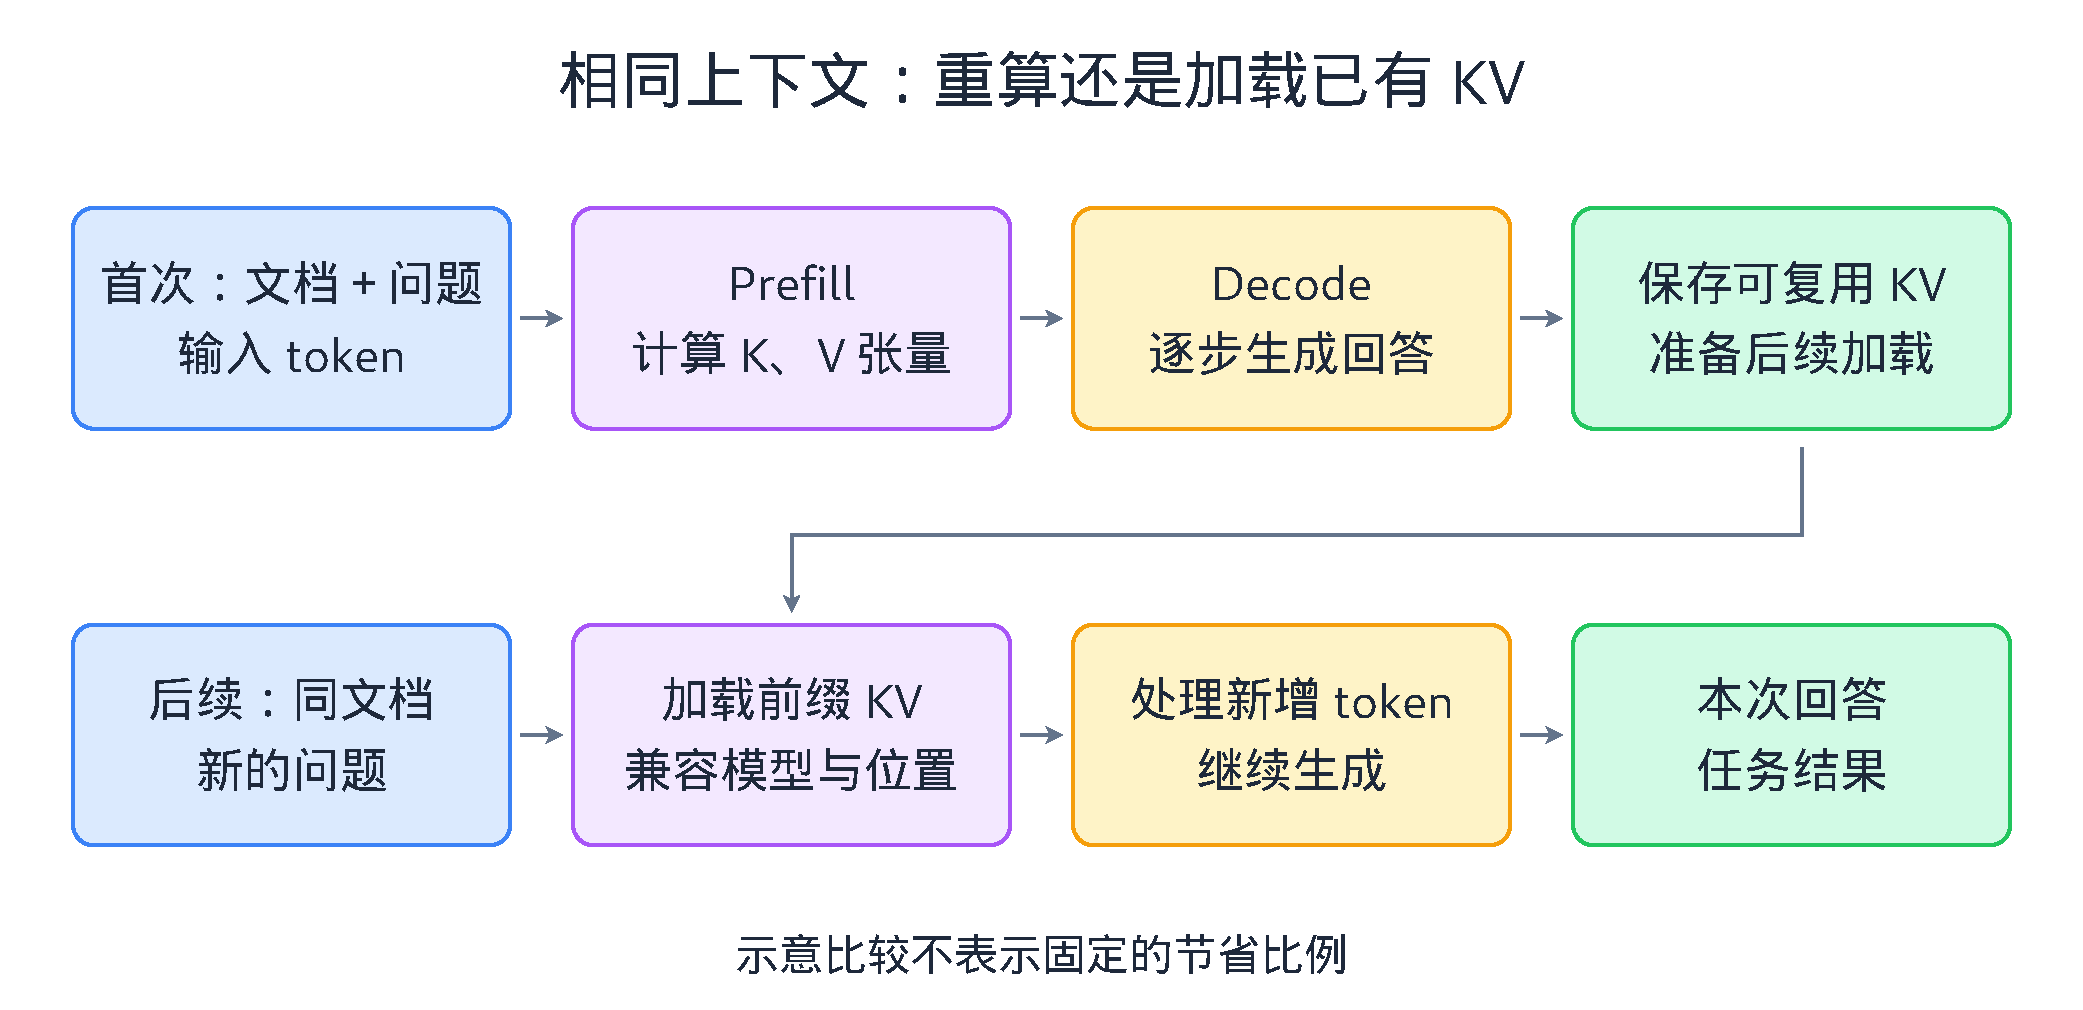
\includegraphics[width=\linewidth,height=.68\textheight,keepaspectratio]{assets/prefill-reuse.pdf}
\caption{相同上下文：重算还是加载已有 KV；依据节目口述整理（01:24:37–01:29:42；01:31:52–01:34:24）}
\end{figure}
\begin{knowledgebox}{读图：第三章 大模型为什么需要缓存自己的计算}
图分为上下两行。上行代表首次请求：从左至右依次为“首次：文档＋问题／输入 token”指向“Prefill：计算 K、V 张量”，再指向“Decode：逐步生成回答”，最后指向“保存可复用 KV：准备后续加载”。下行代表后续请求：最左侧“后续：同文档／新的问题”指向第二个方框“加载前缀 KV：兼容模型与位置”；同时上行最右侧的“保存可复用 KV”有一条折线箭头跨越两行直接连入该方框，随后依次指向“处理新增 token：继续生成”与“本次回答：任务结果”。底部注明“示意比较不表示固定的节省比例”。
\end{knowledgebox}
看清了“保存并加载前缀 KV”对重复计算的替代路径后，接下来的核心工程挑战便是：当这些张量体积巨大且文档块顺序发生变动时，下一章的 LMCache 体系如何把它们高效存下来并灵活复用。
\needspace{6\baselineskip}\subsection{本章小结}
\begin{enumerate}
\item 使用广度推动基础设施演进：2023 年初 ChatGPT 展现出的全民级使用兴趣被江鋆晨判断为 AI 的“互联网时刻”，促使团队在学生推动下转向大模型推理系统研究，并选定体积大、可复用的 KV Cache 作为切入点。
\item 区分人眼感知的输出速度与后台的输入算力开销：用户直接感知的是逐字生成的 Decode 阶段，但在输入远长于输出的智能体与长文档任务中，处理输入的 Prefill 阶段往往占用了很高的 GPU 算力比例，硬件加速 Decode 与软件缓存优化 Prefill 互为补充。
\item 用存储与带宽换取重复计算节省：KV Cache 是注意力机制生成的 K、V 中间张量；在相同模型、相同前缀与兼容配置下将其保存并重新加载，可跳过重复前缀的 Prefill 计算，而实际延迟与成本收益则需综合复用频次、传输带宽与存储开销来权衡。
\end{enumerate}
\needspace{8\baselineskip}\section{第四章 LMCache 如何把研究变成可用的数据层}
明确了KV缓存（KV Cache）避免重复预填充（Prefill）计算的潜力后，下一步挑战是如何将庞大的中间张量在存储与计算节点间高效流转并打破严格前缀匹配的束缚。本章梳理江鋆晨团队从CacheGen、CacheBlend两项核心算法研究出发，在发现工业界缺失独立缓存存储层后开源LMCache的历程，解析多级存储管理机制及解耦架构的工程权衡。
\needspace{6\baselineskip}\subsection{CacheGen：先让大张量更便于传输}
在2023年决定切入大语言模型推理优化时，江鋆晨团队最初的设想是联合数据库、网络与人工智能领域的学者，共同探索他当时称之为“智能体互联网”（Internet of Agents）的研究方向（01:15:59–01:17:04）。在这个构想中，不同专长的团队各自攻关上下文数据库或推理优化，而网络系统出身的江鋆晨团队则将目光锁定在体积最为庞大的KV缓存上。当长上下文生成的KV张量达到数GB乃至数十GB时，如果要将它们保存在外部存储中并在后续请求到达时加载回GPU，首先要跨越的物理瓶颈就是存储空间开销与I/O传输延迟。

如果从外部存储读取并传输KV缓存的耗时，比让GPU把原始文本重新做一遍预填充（Prefill）还要慢，那么缓存复用在系统性能上就失去了意义。正是为了解决“大张量如何存得下、传得快”这一基础问题，团队率先开展了CacheGen项目的研究，专门针对KV缓存做面向存储与网络传输的压缩优化。

作为核心机制解释，CacheGen 根据 KV 张量的分布特征将其编码为更紧凑的比特流（Bitstream）表示，以减小存储与传输体积。同时，借鉴视频流媒体根据网络条件自适应调整码率的思路，CacheGen 将 KV 缓存切分为多个数据块（Chunk），在传输加载时根据当前网络或总线带宽条件动态调整各数据块的压缩级别，或在带宽受限时选择对部分块回退至文本重算，使缓存传输能够适应不同的带宽环境。

通过这种张量编码压缩与按网络条件自适应调整的机制，系统能够显著降低 KV 缓存在存储介质上的空间占用以及跨节点或跨总线传输的带宽压力。在实际工程中，编码与解码本身也会带来一定开销，且有损压缩级别会影响模型输出精度；具体的延迟收益取决于模型规模、上下文长度以及底层的网络或互连带宽条件，需要在压缩率、生成质量与传输耗时之间做平衡。

\needspace{6\baselineskip}\subsection{CacheBlend：越过严格前缀复用的限制}
解决了 KV 缓存的体积与传输问题后，团队紧接着遇到了第二个应用限制：严格的前缀匹配要求。在常规的自回归 Transformer 推理中，当新请求与已缓存内容拥有相同的 Token 前缀时，这部分相同前缀的 KV 缓存可以直接复用；然而在检索增强生成（RAG，先从知识库检索多个相关文档片段再拼接进提示词交由模型回答的技术）或复杂智能体工作流中，系统往往会从数据库里召回 A、B、C 多个独立的文档块，并根据当前问题动态组合它们的先后顺序。

在这些多文档拼接场景下，除了排在最前面的文档块A之外，排在中间或后面的文档块B、C由于前面拼接了不同的内容，其在完整序列中的绝对位置和前序上下文都发生了变化，不再满足“严格前缀一致”的条件。如果因此将B和C全部退回做完整的Prefill重算，那么预先为各个独立文档块生成的KV缓存就无法发挥作用。为了突破这一限制，团队推出了第二个核心研究工作CacheBlend，探索非前缀条件下的KV缓存复用（即访谈中提到的“非前缀复用”或Blending）。

为什么不能把预先单独算好的文档块 A、B、C 的 KV 缓存直接机械拼接（Concatenate）在一起使用呢？从自回归 Transformer 的因果自注意力机制来看，排在后面的词元在计算自身表征时，需要通过自注意力关注排在它前面的文档块词元（即跨片段的因果自注意力依赖），同时模型使用的位置编码（如旋转位置编码 RoPE）也会随词元在拼接序列中的位置改变而变化。如果只是把各自独立计算的 KV 块直接拼起来，文档块 B 和 C 在当初生成缓存时根本“没见过”排在它们前面的文档块 A，缺失了跨片段的注意力交互，可能降低模型生成的回答质量。

CacheBlend 的核心机制是在“全部重算”与“直接拼接”之间找到了一条折中路径：当多个预存的 KV 缓存块被组合在一起时，系统并不是对所有词元一视同仁地跳过计算，而是根据注意力偏差情况，有选择性地挑出少部分对跨片段上下文敏感的 Token 重新计算其键值状态并更新跨片段的因果自注意力，而其余大部分 Token 则直接复用已有的 KV 缓存；同时这少部分 Token 的重算还可以与缓存块的读取传输重叠执行。这种选择性重算少量 Token 的机制，使系统无需从头重算整个长输入，就能以较小的计算代价修复跨片段注意力缺失，保持接近全量重算的生成质量。

\needspace{6\baselineskip}\subsection{先补上缺失的缓存存储系统}
当 CacheGen（压缩传输）和 CacheBlend（非前缀融合复用）的论文相继完成后，江鋆晨满怀信心地走出实验室，去向工业界做技术交流（01:17:04–01:21:47）。他原本的设想很顺畅：既然复用 KV 缓存好处明显，企业应该已经搭好了 KV 缓存存储系统；存了那么多缓存，企业肯定觉得体积太大，正好用上 CacheGen 做压缩；想提高非前缀场景的复用率，正好用上 CacheBlend。于是他在报告时满怀期待地询问接触到的工业界团队，他们的 KV 缓存存储系统在哪里，团队可以帮他们把这些优化算法部署上去。

然而，当时他接洽的这些工业界工程师给出的反馈却让他颇感意外：对方反问什么是 KV 缓存存储系统，并表示他们当时并没有这样的系统。原来，在那个时间点，不少推理引擎虽然在内部使用 KV 缓存，但主要将其视为单次请求生成过程中驻留在 GPU 显存里的临时数据；一旦当前请求生成结束，推理引擎往往就把这些算出来的 KV 张量丢弃了，还没有建立起把它们持久化存下来并跨请求、跨实例调度的外部存储系统。

面对“研究走得比工业界基础设施还超前”的尴尬局面，团队面前只有两条路：要么放弃转化、等工业界自己把存储底座建好后再来推销算法，要么自己动手把缺失的底层系统补上。江鋆晨和学生们等不及工业界慢吞吞地演进，决定亲手打造并开源一套专门用于保存、管理和传输KV缓存的基础设施——LMCache就这样诞生了。这段实践经验表明，LMCache最初并不是为了做一个单纯的存储工程项目而立项，它的初衷是为了给实验室的前沿算法论文提供一个能够在真实世界中运行的系统载体。

作为连接推理引擎与多级存储的中间层，LMCache 支持将需要跨请求复用或 GPU 显存暂存不下的 KV 缓存卸载（Offload）并保存到宿主机 CPU 内存（DRAM，Dynamic Random-Access Memory，动态随机存取存储器，即系统主内存）、本地固态硬盘（SSD，Solid-State Drive，以闪存等固态电子存储芯片阵列制成的硬盘）乃至远端存储系统中，实现跨请求、跨推理实例的提取与共享。随着大模型长上下文应用铺开，越来越多企业开始重视 KV 缓存的持久化管理；据江鋆晨介绍，不少团队直接复用了功能已较完善的 LMCache，有的将其集成后转售（Resell），也有公司围绕 LMCache 与他们展开商业合作。到后来，许多新用户反倒以为他们一开始就是专门为了做存储系统而立项的，忘了团队最初其实是做压缩与非前缀复用算法研究的。

\needspace{6\baselineskip}\subsection{解耦引擎、存储和硬件的代价与价值}
随着大模型产业演进，一个现实的商业与架构问题摆在台面上（01:34:37–01:41:19）：如果未来像 OpenAI 或 Anthropic 这样的头部模型厂商占据了很大市场份额并持续降低 API 价格，或者部分推理引擎与云平台直接在内部集成了缓存功能，为什么行业还会需要 LMCache 这样一个独立的 KV 缓存层？江鋆晨借用流媒体时代的历史经验谈了他的看法：即便 YouTube 和 Netflix 占据了全网很大比例的视频流量，HBO、BBC 等许多公司依然需要服务自有用户、维护各自的视频分发能力；他用“即便少数巨头占去八成需求、剩下那 20\% 谁来做”举例说明，未来仍会有众多 AI 服务商与企业需要部署可控的推理系统。只要这些系统运行的是基于 Transformer 或包含注意力模块的混合架构（Hybrid Model），且需要跨请求、跨层级保存与复用 KV 缓存，就会需要相应的缓存管理层。

在系统架构设计上，嘉宾强调，LMCache追求的是将KV缓存管理变成一个独立的数据层，与上层的推理引擎（如vLLM、SGLang等）、底层的存储介质以及异构的GPU硬件解耦（Decouple）。这里需要准确区分“系统组件解耦”与“模型语义绑定”的界限：解耦是指LMCache不强绑定某一种特定的推理框架、某一家云厂商的存储API或某一款特定芯片；但由于KV张量本身的数值是由特定模型的权重计算得出的，缓存数据在语义上依然与生成它的模型本身相绑定，不能脱离模型权重在不同模型间随意混用。

为什么用户不直接只用某个推理引擎或某朵云内部绑定的缓存，而会需要一个解耦的独立层？因为开源生态与许多企业级基础设施看重的是“保留选择权”与降低厂商锁定（Vendor Lock-in）。除了少数像苹果那样从芯片、系统到应用全部闭环自研的企业外，许多公司在构建 AI 基础设施时，希望能够根据成本和场景更换底层的 GPU 硬件、切换不同的推理引擎或对接不同的存储后端。如果缓存管理与某一个特定引擎或某一种存储后端强绑定，当企业想要替换这些外围组件时，原有的缓存链路就很难直接跨组件平滑迁移和复用。

当然，构建解耦的公共数据层在工程上并不容易。解耦的设计目标是抽象出通用的连接器（Connector）与接口，并力求在不同的引擎、硬件与存储组合下都保持良好的吞吐与延迟表现，避免让用户觉得为了灵活性明显牺牲了性能。江鋆晨坦言，仅靠初创团队自己的工程师，不可能写完适配行业里各类芯片和存储介质的全部集成代码（Integrations）；这项工作需要依靠开源社区与上下游硬件、存储合作伙伴的工程师共同参与建设。同时，在实际生产环境中，引入外部 KV 缓存层的整体收益，始终取决于业务负载的缓存复用频率、从各级存储加载张量的传输开销以及存储介质本身的驻留成本。

\begin{warningbox}{非前缀复用与组件解耦的两个技术前提}
在理解 CacheBlend 与 LMCache 的工作机制时，需要注意区分以下两个技术条件：
\begin{enumerate}
\item 非前缀复用需要修复跨片段因果自注意力：在 RAG 等多文档拼接场景下，排在后面的文档块因前序内容改变而丢失了跨片段注意力关联，同时位置编码也发生变化，因此不能把独立算好的 KV 块直接无损拼接。CacheBlend 通过有选择性地重算少部分关键 Token 来更新跨片段注意力，是在重算开销与生成质量之间做的折中优化。
\item 组件解耦不改变模型语义绑定：江鋆晨在访谈中指出（01:37:59），LMCache 的解耦针对的是推理引擎、运行环境、存储介质和 GPU 硬件等系统组件；而 KV 张量本身是由特定模型的权重计算生成的，缓存复用仍须建立在相同模型（或兼容计算语义）的前提之下。
\end{enumerate}
\end{warningbox}
\begin{knowledgebox}{多级存储卸载（Hierarchical Offloading）的运作方式}
大模型的外部 KV 缓存管理可以类比计算机系统中的多级存储体系。GPU 上的高带宽内存（HBM）访问速度快，但容量昂贵且有限。LMCache 通过连接器挂载在推理引擎旁，可根据缓存策略将需要跨请求保留或 HBM 暂存不下的 KV 缓存分块卸载到容量更大、单位成本更低的存储层级中——包括宿主机 CPU 内存（DRAM，与 GPU 之间通过 PCIe 或特定平台的芯片互连总线传输）、本地固态硬盘（SSD），以及跨节点的远端存储系统。当后续请求命中已缓存的上下文片段时，系统再通过连接器将对应的 KV 张量流式加载回 GPU 显存，从而用存储容量与传输带宽换取重复 Prefill 计算的节省。
\end{knowledgebox}
\begin{table}[H]\centering\small
\caption{从学术论文到开源系统的核心模块对比}
\begin{tabular}{>{\raggedright\arraybackslash}p{\dimexpr(\linewidth-6\tabcolsep)/3\relax}>{\raggedright\arraybackslash}p{\dimexpr(\linewidth-6\tabcolsep)/3\relax}>{\raggedright\arraybackslash}p{\dimexpr(\linewidth-6\tabcolsep)/3\relax}}
\toprule
技术/系统名称 & 针对的核心痛点 & 核心机制与工程实践关系\\\midrule
CacheGen & KV张量体积过于庞大，跨网络或总线传输及外部存储的带宽与空间开销过高 & 根据 KV 张量分布定制编码以压缩成紧凑比特流，并结合当前网络或传输带宽条件动态选择分块压缩级别或局部重算\\[4pt]
CacheBlend & RAG与多文档拼接场景下，排在后面的文档块因前序内容改变而无法满足严格前缀匹配 & 在组合多个预存 KV 块时，有选择性地重算少部分关键 Token 以更新跨片段因果自注意力，突破仅限严格前缀复用的限制\\[4pt]
LMCache & 早期推理引擎在单次请求结束后即丢弃KV缓存，工业界缺乏跨请求、跨实例的持久化缓存管理底座 & 最初为承载团队算法论文而开源的系统，现已演进为连接vLLM/SGLang等引擎与CPU/SSD/远端存储的独立KV缓存数据层\\[4pt]
组件解耦架构（Decoupled Layer） & 企业替换推理引擎、GPU芯片或存储后端时，强耦合的内置缓存方案会导致迁移困难与厂商锁定 & 通过开源社区与硬件/存储厂商共建连接器（Connector），将KV管理与运行环境、存储介质和硬件解耦，赋予用户组合基础设施的自由\\[4pt]
\bottomrule\end{tabular}\end{table}
为了让实验室里的压缩与非前缀复用算法真正跑在生产环境中，江鋆晨团队开源了 LMCache，将其打造为解耦上层推理框架与底层多级存储介质的公共数据层。下图展示了这一承上启下的系统位置。
\begin{figure}[H]\centering
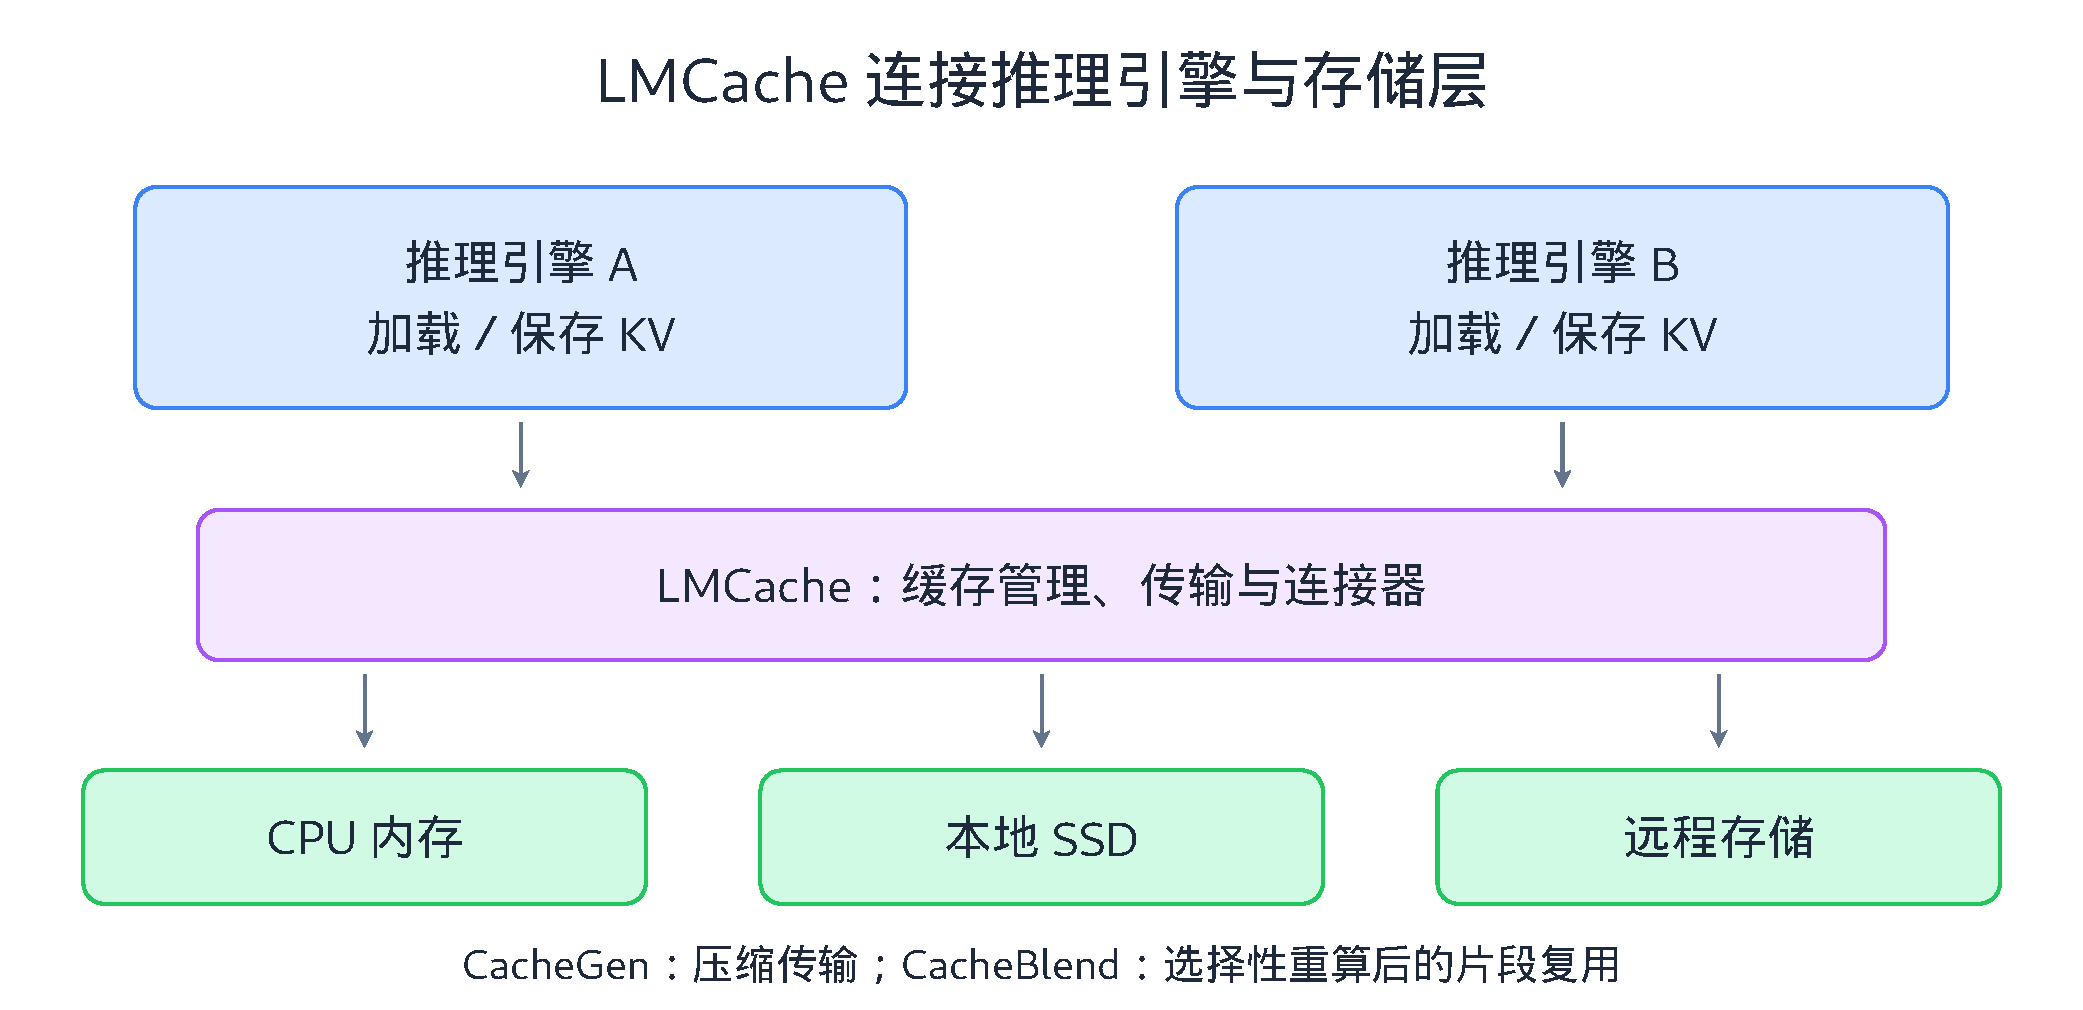
\includegraphics[width=\linewidth,height=.68\textheight,keepaspectratio]{assets/cache-layer.pdf}
\caption{LMCache 连接推理引擎与存储层；依据节目口述整理（01:15:59–01:21:03；01:37:28–01:40:55）}
\end{figure}
\begin{knowledgebox}{读图：第四章 LMCache 如何把研究变成可用的数据层}
图上方并列“推理引擎 A：加载／保存 KV”与“推理引擎 B：加载／保存 KV”两个方框，各自通过向下的箭头接入中间横跨全局的宽框“LMCache：缓存管理、传输与连接器”。从中间层再向下分出三条箭头，分别指向底部的三个存储方框：“CPU 内存”、“本地 SSD”和“远程存储”。图最下方一行小字标出了两项核心算法定位：“CacheGen：压缩传输；CacheBlend：选择性重算后的片段复用”。
\end{knowledgebox}
当这层连接推理引擎与多级存储的缓存底座搭建完毕后，KV 缓存在系统里就不再只是转瞬即逝的临时变量；下一章我们将探讨它在智能体多轮交互中如何演进为模型运行期记忆的管理通道。
\needspace{6\baselineskip}\subsection{本章小结}
\begin{enumerate}
\item 算法先行突破传输与复用限制：团队先后通过 CacheGen（根据 KV 分布定制编码并按带宽条件自适应传输）缓解大体积张量的传输瓶颈，通过 CacheBlend（选择性重算少量 Token 以恢复跨片段因果自注意力）突破严格前缀匹配的限制。
\item 补齐外部缓存管理底座：在早期向工业界介绍算法时，团队发现当时接洽的系统往往在请求结束后就丢弃 KV 缓存、尚无外部持久化存储层，遂开源 LMCache 来承载算法研究，并逐步发展为支持 CPU 内存、本地 SSD 与远端存储的多级缓存管理层。
\item 推进组件解耦与社区共建：LMCache 致力于将 KV 缓存管理与推理引擎、存储介质及硬件解耦（同时保留模型层面的计算语义兼容），通过与开源社区及上下游厂商共建连接器，帮用户在系统灵活性、加载开销与复用收益之间取得平衡。
\end{enumerate}
\needspace{8\baselineskip}\section{第五章 Agent 记忆的三条改进路径}
当LMCache建立起跨层级的KV缓存数据层后，一个更深远的问题随之浮现：在高频交互的智能体（Agent）时代，缓存除了用来跳过重复计算以节省成本，还能发挥什么作用？本章梳理智能体多轮交互带来的上下文复杂性，对比改进AI能力的“修改权重、组织提示词、管理内部状态”三条互补路径，并探讨如何将“模型原生记忆管理”的长期愿景转化为扎实的研究问题。
\needspace{6\baselineskip}\subsection{多轮行动为什么放大了上下文问题}
近年来，以编程智能体（Coding Agent，能够读取代码库、调用工具并辅助编写与测试代码的 AI 系统）为代表的智能体应用备受关注（01:41:19–01:44:45）。江鋆晨认为，智能体展现出的能力，既源于基座模型本身的支持，也离不开与环境的多轮交互。如果只调用模型一次，模型的潜力往往还没有充分发挥；而智能体通过在完成任务的过程中与外部环境、工具进行多轮交互，获得了更强的适应性，从而把模型解决复杂任务的能力进一步发挥出来。

与此同时，多轮交互也显著增加了上下文与记忆管理的复杂度。在完成一项长周期任务的过程中，智能体需要记住的内容随着交互次数增加而不断变多；而且记忆管理并不是简单地把所有历史内容原样堆砌在一起，往往需要根据当前任务不停地筛选、组织甚至重排（Shuffle）上下文，提取出最相关的记忆，并决定哪些内容应该放在前面、哪些放在后面。

目前工业界大多数记忆管理模块，都是在“人类可读的符号层”处理信息——也就是直接管理自然语言文本、代码片段或图片。江鋆晨结合自己使用 ChatGPT 个性化记忆（Memory）功能的日常体验，举了一个让他觉得有些困扰的例子：因为他之前曾和 ChatGPT 讨论过自己创立的 Tensormesh 公司的事，结果后来当他询问完全无关的其他日常事务建议时，ChatGPT 还是会冷不丁地在回答里把话题扯回 Tensormesh 上。这个个人体验直观地说明，在多轮交互中如何准确把握历史记忆的“相关性”并避免无关上下文的干扰，依然是当前记忆管理需要解决的实际难题。

与在表层管理自然语言文本不同，江鋆晨团队关注的是人类语言在模型内部计算空间中的“镜像”——即模型在预填充（Prefill）阶段生成的KV缓存状态。如果说文本管理是在替模型整理人类看得懂的笔记本，那么KV缓存管理则是直接深入模型运行时的内部状态空间，去调度那些只有模型自己能直接读取的中间张量。

\needspace{6\baselineskip}\subsection{修改权重、组织上下文、管理内部状态}
为了说明 KV 缓存管理在 AI 技术体系中的位置，江鋆晨在访谈中将大家改进 AI 系统表现的常见思路归纳为三条路径（01:44:50–01:47:50）。第一条路是训练模型（Train Model），即通过改变模型权重（Model Weights）来训练出能力更强的新模型；第二条路是组织上下文与应用编排（Context / Prompt Engineering），即在给定模型的前提下，通过改进提示词、检索与上下文输入来发挥模型的潜力。

江鋆晨团队探索的则是位于二者之间的“第三条路”：针对一个已经训练好的模型和已经写好的应用程序，直接去存储、尝试理解并优化模型在运行过程中生成的内部记忆状态（即 KV 缓存）。在这三条路径的划分中，第一条路改变的是模型参数权重，第二条路改变的是表层的输入上下文，而第三条路操作的是推理时的内部注意力状态。

在个性化（Personalization）或智能体自我改进（Self-Improvement，指系统在交互过程中不断改进后续任务表现）等目标下，为什么这三条路径各有分工？从机制上看，模型训练与微调（包括轻量微调方法）能够把通用能力或领域知识沉淀到权重参数中，但通常不直接用来承载每个用户在每次实时会话中动态变化的上下文状态；上下文工程在应用层直观灵活，而且在前缀或片段兼容时本身也可以配合 KV 缓存复用，但它操作的对象始终是表层的文本或符号；而直接管理与优化内部 KV 状态，则试图在跳过重复 Prefill 计算的同时，从模型原生的张量表征层面去分析与调整上下文记忆。

因此，江鋆晨认为，训练模型权重、组织上层上下文与管理底层 KV 缓存这三条路并不是互相排斥的替代关系，而是互补的。在构建面向个性化或自我改进的智能体系统时，这三种思路完全可以结合使用、协同演进。

\needspace{6\baselineskip}\subsection{从避免重算到理解和选择记忆}
明确了第三条路径的定位后，就可以看清 Tensormesh 与 LMCache 在当前落地业务与长远研究愿景上的区分（01:29:42–01:31:14）。在现阶段，为了解决企业客户最迫切的实际痛点——即高昂的 Token 计算成本与长上下文处理耗时，KV 缓存管理最直接、最易落地的价值是“避免重复计算”：把模型读过的代码库或长报告以 KV 缓存的形式存下来，下次直接加载复用，从而省去重复的 Prefill 算力开销。

在此基础上，江鋆晨在访谈中阐述了团队更长远的研究愿景：如果把 KV 缓存视为模型对已读上下文形成的内部记忆，那么除了原样保存和复用之外，未来能否进一步去“理解”和“优化”这段记忆？例如，通过分析模型运行时的内部状态，看看模型对哪些 Token 的注意力更集中、觉得哪些内容更重要；甚至进一步研究如何对 KV 缓存做筛选或优化，让模型在后续生成时把注意力放在更相关的上下文上，从而改善生成行为，而不是对所有杂乱输入做一个平均化的处理。

从 Transformer 的注意力计算机制来看，这里可以做一个清晰的技术区分：首先，保存并跨请求复用 KV 张量以节省重复计算，已经是 LMCache 落地实现的工程能力；而通过分析、筛选或调整 KV 状态来改善智能体记忆与生成行为，则是团队正在推进的研究方向与长期愿景。其次，在注意力机制中，模型对不同历史词元的关注程度（注意力权重，Attention Weights）是由当前查询向量（Q）与历史键向量（K）做点积并经过 Softmax 归一化后动态算出的，K、V 张量本身提供的是计算注意力的键值表征，并不能不经计算直接当作明文读出，对 KV 状态的筛选、裁剪或重加权也需要通过具体下游任务的生成质量评测来检验效果。

在江鋆晨看来，过去许多专门做模型训练的人不怎么关注推理底层的 KV 缓存，而不少做推理和应用的人又觉得 KV 缓存只是单次生成完就可以丢掉的临时数据、是一堆看不懂的浮点数。正因为这一层处于模型训练与上层提示词工程之间的交叉地带，把重要上下文沉淀为可存储、可复用的 KV 缓存，并进一步探索其分析与优化空间，才成了他们眼中很有吸引力的研究与创业方向。

\needspace{6\baselineskip}\subsection{把原生记忆愿景变成具体研究问题}
当主持人顺着这一愿景追问“是否意味着所有能存储的KV缓存都应该被永久保存下来，用于下一代模型或范式的提升”时，江鋆晨给出了审慎的修正（01:48:15–01:50:54）。他指出，“把所有KV缓存全部存下来”的说法过于极端；更准确的表述是，任何被用户或系统判定为“重要的上下文”（Important Context），都值得被转化为KV缓存的形式妥善保存与管理。

这一界定对应的工程逻辑很清晰：在真实的应用场景中，日常交互会产生大量一次性或无关紧要的对话内容，如果不加筛选地把所有 KV 状态全部永久存下来，既会占用过多存储资源，也容易像前文提到的聊天记忆例子那样引入无关历史的干扰。因此，围绕模型内部状态做记忆管理，核心在于研究“哪些重要上下文值得存为 KV 缓存、如何高效存取、以及如何在后续任务中合理复用与优化”。

将这一宏大愿景拆解到计算机系统与人工智能交叉的具体科研与工程议题上，未来的探索可以归纳为三个循序渐进的层次：

• 状态的选择与生命周期管理：如何结合上下文语义与注意力分布指标，自动识别哪些长文本或交互历史属于高价值上下文，并在多级存储（GPU/CPU/SSD/远端存储）中制定合理的缓存留存、淘汰与更新策略。
• 跨片段的状态融合与相关性控制：当智能体从记忆池中调取多个历史KV块时，如何利用类似CacheBlend的选择性重算或注意力校准机制，让不同时期的内部状态平滑融合，同时抑制无关历史状态对当前任务的干扰。
• 面向自我改进的状态压缩与提炼：如何将长周期交互产生的庞大KV张量提炼为更紧凑的内部表征，并建立量化的评测基准，验证经过状态优化后的KV缓存能否在保证生成精度的前提下，实质性提升智能体在复杂任务上的表现。

\begin{warningbox}{缓存保存了什么，选择与优化记忆还需要什么}
在理解“将 KV 缓存作为模型运行期记忆来管理”时，可以从机制上区分已落地的能力与进一步的研究方向：
\begin{enumerate}
\item KV 缓存保存的是运行期上下文状态，而非模型权重：保存 KV 缓存是指留存特定输入序列在各层自注意力中的键值张量，以便在兼容条件下加载复用、跳过重复 Prefill；它并没有修改模型的参数权重（Model Weights）。
\item 从 K、V 张量到注意力关注度需要结合查询计算：模型在生成时对哪些历史 Token 更关注，取决于当前步的 Query 与缓存中 Key 的注意力计算结果。因此，想要在保存复用之上实现“筛选重要记忆”或“调整状态以改善生成行为”，还需要设计专门的状态评分、片段融合与评测机制。
\item 聚焦重要上下文而非无差别全量存储：江鋆晨在访谈中说明（01:49:22），愿景并不是把所有临时生成的 KV 缓存都永久存下来，而是将用户或系统认定的“重要上下文”转化为 KV 缓存形式妥善管理。
\end{enumerate}
\end{warningbox}
\begin{importantbox}{为什么内部状态管理能与权重训练、上下文工程互补}
如果从操作对象的层级来看 AI 系统的改进方式：底层是模型权重（通过预训练、微调或强化学习更新参数，负责提供基础推理与领域能力），顶层是上下文与提示词工程（在应用侧检索、筛选和编排文本或代码，灵活组织每次任务的输入，且在前缀匹配时也可结合缓存复用），而中间层则是模型推理时生成的内部状态（KV Cache）。这一中间层把顶层输入的重要文本转化成了底层模型可直接读取的键值张量——在工程上，它通过跨请求持久化避免了相同上下文的重复 Prefill 计算；在研究上，它为跨片段融合（如 CacheBlend）以及后续的状态筛选与优化提供了直接的操作对象。
\end{importantbox}
\begin{table}[H]\centering\small
\caption{提升智能体（Agent）与大模型能力的三条互补路径对比}
\begin{tabular}{>{\raggedright\arraybackslash}p{\dimexpr(\linewidth-8\tabcolsep)/4\relax}>{\raggedright\arraybackslash}p{\dimexpr(\linewidth-8\tabcolsep)/4\relax}>{\raggedright\arraybackslash}p{\dimexpr(\linewidth-8\tabcolsep)/4\relax}>{\raggedright\arraybackslash}p{\dimexpr(\linewidth-8\tabcolsep)/4\relax}}
\toprule
改进路径 & 核心操作对象 & 解决的核心问题 & 机制特点与实践局限\\\midrule
第一条路：模型训练与微调（Model Training） & 模型的权重参数（Model Weights） & 提升基座模型的通用推理能力，或将领域知识固化到参数中 & 通过预训练、微调（含轻量微调）或强化学习更新参数；适合沉淀通用或领域能力，但通常不直接用于承载每次实时会话的动态上下文\\[4pt]
第二条路：上下文与提示词工程（Context Engineering） & 人类可读的输入文本、代码与提示词（Prompts） & 在不改权重的前提下，通过动态检索、拼接与重排文本激发模型潜力 & 直观灵活，是当前智能体记忆管理的主流做法，也可配合前缀缓存使用；但仅在符号层管理长文本仍受限于重复输入处理与相关性筛选难题\\[4pt]
第三条路：内部状态与KV缓存管理（Internal State Management） & 模型运行期生成的注意力键值张量（KV Cache） & 将重要上下文保存为模型可直接加载的中间状态，避免重复计算并探索状态级的分析与优化 & 保存与复用已可有效减少重复 Prefill 开销；进一步的状态理解、筛选与优化属于研究方向，需结合多级存储、跨片段融合与下游任务质量评测\\[4pt]
\bottomrule\end{tabular}\end{table}
面对智能体在复杂任务中的个性化与自我改进需求，工程界与学术界正在从不同层面寻找突破口。江鋆晨在访谈中将现有的技术手段归纳为三条互补路径，下图展示了这三者在系统中的分工与共同目标。
\begin{figure}[H]\centering
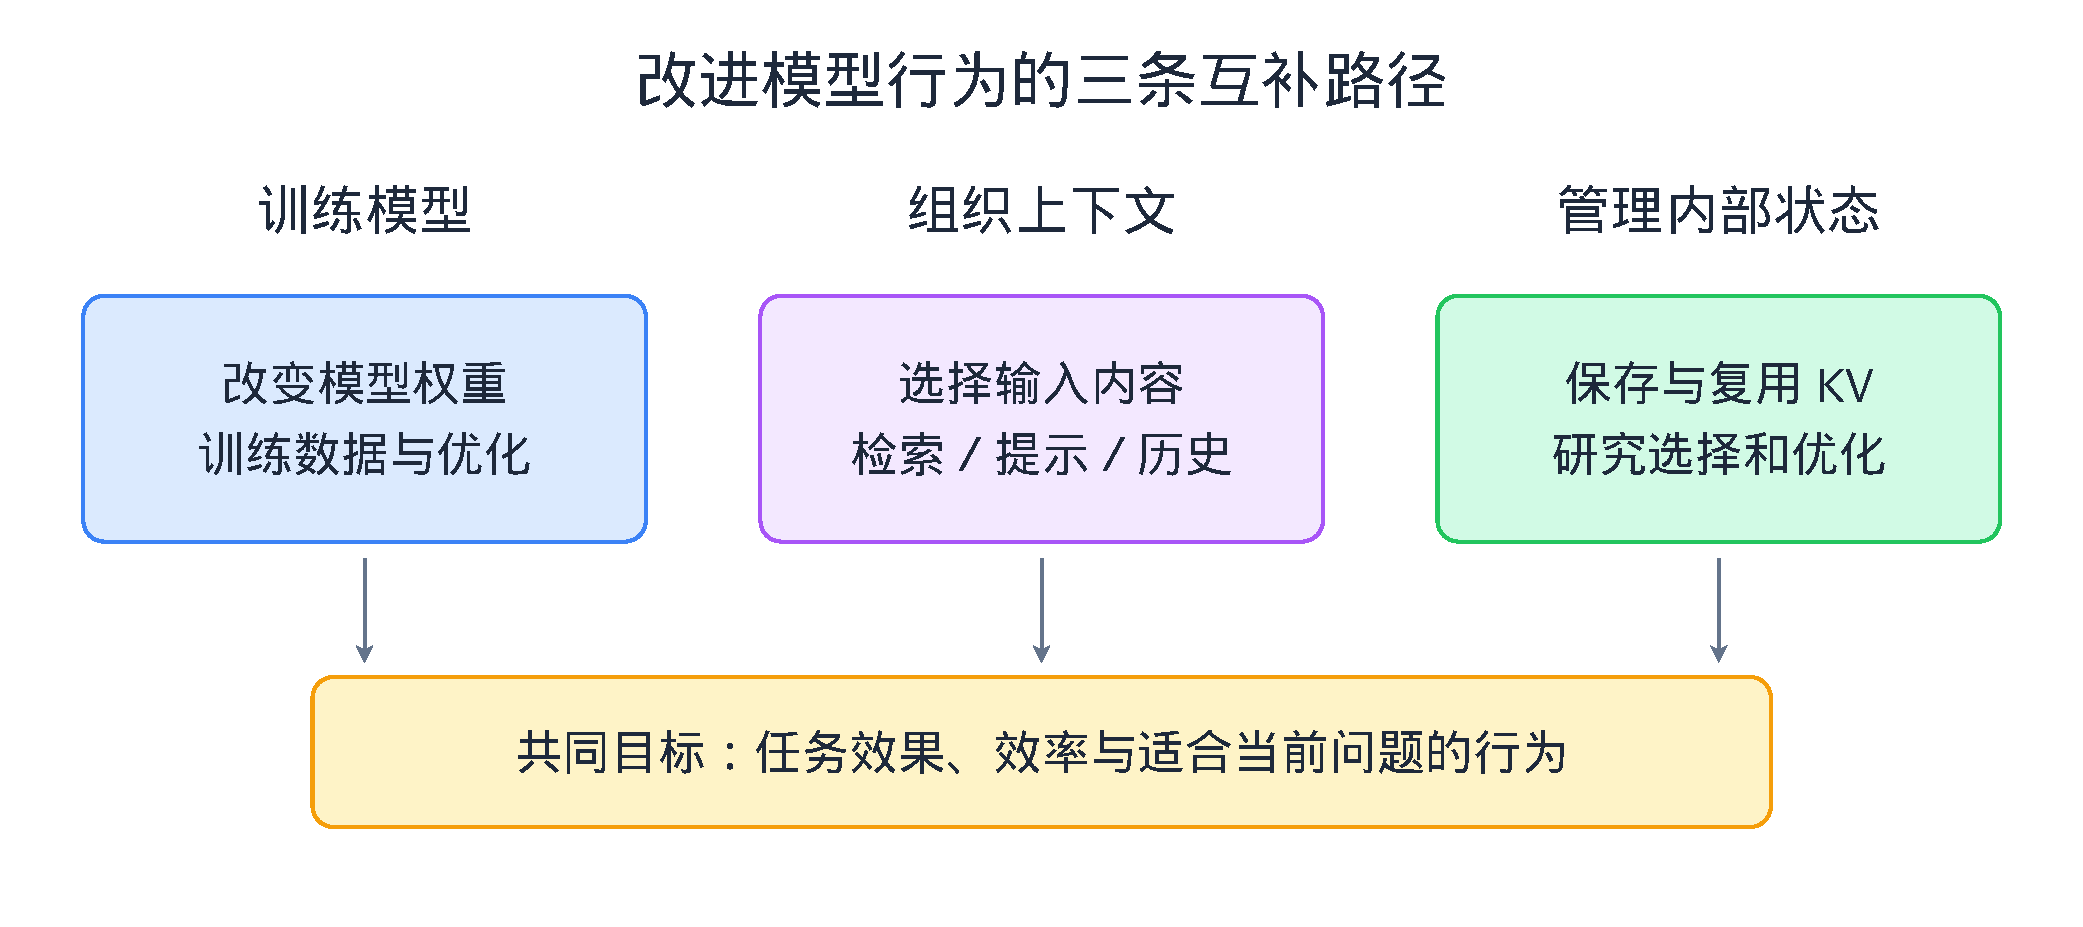
\includegraphics[width=\linewidth,height=.68\textheight,keepaspectratio]{assets/memory-paths.pdf}
\caption{改进模型行为的三条互补路径；依据节目口述整理（01:41:55–01:49:22）}
\end{figure}
\begin{knowledgebox}{读图：第五章 Agent 记忆的三条改进路径}
图上方由左至右并列三列。左列标题为“训练模型”，下方方框写着“改变模型权重／训练数据与优化”；中列标题为“组织上下文”，下方方框写着“选择输入内容／检索／提示／历史”；右列标题为“管理内部状态”，下方方框写着“保存与复用 KV／研究选择和优化”。三列方框底部各有一条向下的箭头，共同指向下方横跨全局的汇总长框：“共同目标：任务效果、效率与适合当前问题的行为”。
\end{knowledgebox}
明确了内部状态管理作为“第三条路”的学术与工程定位后，要想把这套技术底座真正推向全行业并持续迭代，研究团队自身也必须经历从高校实验室向商业初创公司的组织跨越，这正是下一章的主题。
\needspace{6\baselineskip}\subsection{本章小结}
\begin{enumerate}
\item 多轮交互带来复杂的上下文管理需求：智能体通过与环境进行多轮交互发挥了模型处理复杂任务的能力，但也使需要管理的历史信息不断累积，如何筛选和重排相关记忆、避免无关历史干扰成为关键挑战。
\item 改进 AI 表现的三条互补路径：访谈将常见改进思路归纳为“改变模型权重”、“组织输入上下文”与“管理模型内部状态（KV 缓存）”三条路径；三者操作层级不同，在个性化与自我改进等目标下互为补充。
\item 从避免重复计算走向重要上下文的状态管理：保存与加载 KV 缓存已在工程上用于减少重复 Prefill 计算、降低成本；而将重要上下文转化为 KV 缓存并进一步研究如何分析、筛选和优化这些内部状态，则是团队长期探索的研究愿景。
\end{enumerate}
\needspace{8\baselineskip}\section{第六章 从开源研究组到有节奏的创业团队}
当LMCache从一个承载学术论文想法的开源工具演变为工业界广泛接入的基础设施，高校实验室的组织形式便遇到了天然边界。本章梳理江鋆晨与学生创立Tensormesh的现实动因，探讨学者在接触风险投资与算力巨头时的认知转换，分析在缺乏论文截稿日与直接竞品的早期赛道上如何保持工程节奏，以及师生如何转化为平等互信的联合创始人。
\needspace{6\baselineskip}\subsection{学生毕业后谁来维护生产系统}
一个高校实验室为什么要跨越学术边界，把开源项目变成一家商业公司？在访谈中，江鋆晨谈到了两个很现实的原因（01:19:21–01:24:21）。第一个直接原因是高校研究组的人员流动：当时参与开发 LMCache 的主力博士生很快就要毕业了。对于这个主要由几个博士生搭建起来的项目而言，如果不出来创业组建团队，一旦核心学生毕业离校，项目就面临难以持续推进和维护的现实困境。

第二个原因在于构建工业级基础设施（Infra）并持续转化科研成果的体量要求。江鋆晨坦言，以一个高校研究组的力量去打造一套希望被工业界广泛采用的开源基础设施，回头看其实风险很大——工业界大公司早晚会意识到 KV 缓存管理的需求，届时他们既可能借鉴思路，也可能直接投入大团队自行开发。LMCache 之所以能抢出时间窗口，是因为团队在工业界尚未普遍发力这一层时就把功能做得比较完善了。但当越来越多企业开始在生产环境中直接复用、转售 LMCache 或寻求商业合作时，对于他们团队的目标——既要给工业界提供可靠的大型基础设施，又要将实验室论文里的研究想法源源不断地输送到产业一线——单靠学校实验室或单纯维持一个校园开源项目已无法胜任。因此，对他们而言，成立公司、引入风险投资（Venture Capital，简称 VC，向初创企业提供资金支持并换取股权的投资机构）并招募全职团队成了必须要走的一步。

围绕创业初期的节奏，江鋆晨还分享了他们团队的一段亲身经历：创业第一天未必要立刻搬到硅谷。在 Tensormesh 成立的前半年，团队一共只有不到七八个人，全部由江鋆晨和他在芝加哥大学的学生组成。在这个磨合早期核心产品的阶段，留在芝加哥其实完全可以运转，他回想起来觉得前半年搬去硅谷有点太早了。但当公司走过最初期、进入当前需要招募优秀人才、接触重要客户以及获取一线行业信息的阶段，搬到硅谷对他们来说就变得非常关键了。

\needspace{6\baselineskip}\subsection{为不同利益方解释同一项技术}
从高校学者转型为初创公司CEO，江鋆晨坦言自己像被“直接丢进大海里学游泳”，其中最陌生的一课就是与投资人打交道（01:50:54–01:53:27，01:55:44–02:00:24）。在学术界十几年，研究者习惯了面对同行评审，却几乎从未接触过风险投资人。江鋆晨回忆，第一次接触投资人是由博士导师张辉帮忙引荐的；起初聊了几次，他甚至都没意识到对方已经在考察和“面试”自己，还在张辉的提醒下才开始专门打磨项目路演（Pitch，向投资人简明阐述商业与技术逻辑的演示）。当这位投资人专门飞到芝加哥与几位联合创始人见面时，江鋆晨起初只打算在学校旁边的咖啡馆随便聊聊，还是张辉在电话里及时提醒他这太不正式，至少要找个房间做一场完整的演示。

到了真正拿到投资意向书（Term Sheet，投资人与创业公司就估值、投资额及核心权利义务达成初步意向的法律文件）的那一刻，所有的财务与法务条款对学者而言都是全新概念，他不得不连夜给张辉和律师打电话请教如何理解条款与谈判。节目披露，Tensormesh在约八个月内先后完成了两轮融资，近期一轮融到了2000万美元（注：这是外部股权融资额，不等同于公司的商业营收）。江鋆晨总结说，熟悉学术界创业者的早期投资人往往抓大放小——他们清楚教授们不懂融资套路，只要底层技术确实切中了未来的核心痛点，投资人并不介意创始人在商务形式上的生疏。

更具代表性的是产业资本的动向：在Tensormesh的融资阵容中，同时出现了英伟达（NVIDIA）与超威半导体（AMD）这两家在GPU硬件市场上激烈竞争的巨头。为什么互为对手的芯片厂商会分别独立地决定投资同一家软件初创公司？江鋆晨解释，两家公司在接洽之初并非跟风，而是各自独立地对技术趋势达成了同一个判断——要让自家的硬件算力在长上下文推理中发挥出最高效率，中间必须有一层极其高效的KV缓存存储与传输层。当然，巨头参与投资并达成技术共识，并不意味着他们会停止内部的自研探索，也不代表为某款软件提供排他性的商业担保；他们选择投资，是因为认可这一基础设施方向对释放硬件潜能的关键作用，希望与生态中跑在前面的团队共同把技术做通。

\needspace{6\baselineskip}\subsection{没有论文截止日，怎样和自己赛跑}
拿到融资、组建团队之后，创业日常中最难适应的心理落差是什么？江鋆晨给出的答案是：在缺乏外部强制时间表和直接同业对手的阶段，如何激励团队“跟自己赛跑”（01:53:27–01:55:44）。在学术界做研究，时间节奏是由一个个顶会的论文截稿日（Paper Deadline）切割出来的——赶不上截稿日，论文就投不出去，这种明确的外部倒计时天然推着所有人冲刺。而在大模型推理引擎等赛道，几家知名开源项目之间存在贴身肉搏的正面竞争，对手的每一次版本发布也是强大的外部鞭策。

相比之下，按江鋆晨当时的观察，Tensormesh 所在的独立 KV 缓存层方向，在创业初期还没有出现直接对标的同类型创业公司；虽然有些大公司内部的工程小组会为了证明团队自身价值而做一些相关尝试，但尚未形成直接的正面市场竞争。既没有论文截稿日，又缺少紧咬在身后的直接竞争对手，团队面临的最大考验就是如何在内部给自己施加足够的推力。

为此，江鋆晨和团队始终保持着强烈的紧迫感。他在访谈中给出了自己当时的一个笃定预判：等到大家都意识到 KV 缓存这件事的重要性时——他个人估计可能不需要一年时间——各大公司都会纷纷推出 KV 缓存相关的产品。在他看来，初创团队必须趁着巨头全面入场前抓紧窗口期，把系统性能和生态做得足够扎实，争取届时至少能与大公司平起平坐甚至保持领先。因此，从学者转变为创业者，必须学会在没有外部截稿日的情况下，依靠这种危机感和阶段性的产品交付目标来激励团队“跟自己赛跑”。

\needspace{6\baselineskip}\subsection{师生联创如何成为平等的决策关系}
Tensormesh 的另一个鲜明特点是“师生联创”——江鋆晨与他指导的毕业博士生共同作为联合创始人（Cofounder）全职创业，研究组里参与早期贡献的其他学生也获得了原始股（02:00:25–02:04:35）。谈及这种组合，江鋆晨分享了他基于身边同背景学者创业案例的个人观察：在他认识的同领域老师里，创业时没有拉上自己学生一起做的，后来大多不太顺利；当然他也专门说明，这只是他身边的小样本观察，没有统计普遍性，业界也有不少老师不带学生、而是聘请职业经理人（Professional CEO）把公司做成功的例子。就他自己的体验而言，做技术创业时和学生一起干有一个先天的磨合优势：双方在博士阶段的长期科研合作中已经建立起稳定的信任结构——学生相信导师对长远技术愿景（Vision）的判断，导师则充分信任学生的技术实力与执行力。

不过，一旦从实验室走向公司，原有的师生上下级关系就必须转换为平等的合伙人关系。在真实的产品研发与架构演进中，导师提出的设想不可能永远正确。当联合创始人们发生分歧，甚至事后证明是学生对了、老师错了的时候，团队该如何决策？

江鋆晨用日常研发中的技术反对意见（Pushback）解释了这种互动方式。有时他会提出一些比较激进的技术想法，而作为联合创始人的学生会直接从技术角度提出异议，指出这个想法在当前工程条件下还做不了。遇到这种情况，江鋆晨会相信并尊重学生的技术判断。这种顺畅沟通的基础在于双方的信任：导师知道学生说“现在做不了”，是基于真实的技术评估，而不是因为不认同公司方向而找借口敷衍；学生也清楚导师提出想法是为了探索长期价值，双方可以坦诚地把当前条件尚不成熟的想法先放一放，留待日后再讨论。正是这种保留科研合作信任、在公司内部平等讨论技术可行性的关系，让师生联创团队在创业初期得以顺畅配合。

\begin{knowledgebox}{学者创业的基础商业概念：VC、Pitch 与 Term Sheet}
对于习惯了申请科研基金（Grant）和发表论文的高校研究者而言，进入创业赛道需要了解一套不同的沟通与法律概念：
• 风险投资（Venture Capital，简称 VC）：向具有成长潜力的初创企业提供股权资金支持的投资机构。与侧重学术创新的科研基金不同，早期科技投资人既看重底层技术的独特性，也关注其能否转化为商业与生态价值。
• 项目路演（Pitch）：创始人向投资人清晰阐述“解决什么问题、技术为何重要、团队具备什么优势以及未来发展方向”的演示与沟通。
• 投资意向书（Term Sheet）：投资方表达投资意向时出具的框架性条款文件，通常包含估值、投资额、优先清算权等经济条款，以及董事会席位、投票权等治理与控制条款（其中多数投资条款通常为非约束性意向，保密与排他期等条款可能具有法律约束力）。签署 Term Sheet 后，双方一般还需推进尽职调查与正式法律文件的谈判交割。
\end{knowledgebox}
\begin{importantbox}{师生联创团队如何实现从科研指导到平等决策的转换}
在高校技术成果转化中，“教授+核心博士生”是常见的初创班底。结合江鋆晨团队的实践，这种结构的有效运转依赖三个要素：
\begin{enumerate}
\item 前期磨合红利：师生在读博期间已经共同经历过课题探索与系统搭建，省去了陌生合伙人之间漫长的能力验证与性格磨合期。
\item 角色切换与平等决策：在学校里导师负责指导与把关；在公司里，联合创始人之间是平等的伙伴关系。导师需要放权，尊重学生在具体工程实现与技术可行性上的反对意见（Technical Pushback）。
\item 区分愿景与当期执行：当一线工程团队否决某项激进功能时，健康的团队能区分“长期方向错误”与“当期工程条件不成熟”，从而在不伤害长期愿景的前提下做出务实的排期取舍。
\end{enumerate}
\end{importantbox}
\begin{table}[H]\centering\small
\caption{高校开源研究组与商业初创公司的运作机制对比}
\begin{tabular}{>{\raggedright\arraybackslash}p{\dimexpr(\linewidth-8\tabcolsep)/4\relax}>{\raggedright\arraybackslash}p{\dimexpr(\linewidth-8\tabcolsep)/4\relax}>{\raggedright\arraybackslash}p{\dimexpr(\linewidth-8\tabcolsep)/4\relax}>{\raggedright\arraybackslash}p{\dimexpr(\linewidth-8\tabcolsep)/4\relax}}
\toprule
维度 & 高校开源研究组（Academic Group） & 商业技术初创公司（Tech Startup） & 转型期的核心挑战与应对\\\midrule
人员与维护周期 & 以博士生为主力，随毕业周期自然流动，难以长期承担生产级系统的日常维护 & 通过融资组建全职工程与支持团队，保障系统长期演进与企业级服务可靠性 & 在核心学生毕业前完成公司化落地，避免开源项目因人员毕业而断档\\[4pt]
时间节奏与驱动力 & 由学术会议的论文截稿日（Paper Deadline）切分阶段，外部时间节点明确 & 没有固定截稿日；在细分赛道尚无直接竞品时，缺乏显性的外部倒计时 & 依靠对行业大厂入场窗口的预判，“与自己赛跑”，建立内部工程迭代节奏\\[4pt]
资源获取与沟通对象 & 撰写基金申请书或学术论文，向同行学者证明方法的理论与实验新颖性 & 通过路演（Pitch）与客户对接，向投资人和产业方证明系统降本增效的商业与生态价值 & 学者需快速补齐商业沟通、投资意向书（Term Sheet）谈判及产业协同能力\\[4pt]
团队协作与决策关系 & 导师指导学生，以探索未知问题、完成学位论文与学术发表为目标 & 联合创始人平等共事，以产品落地与公司生存发展为共同目标 & 保留师生间对长期愿景与技术实力的互信，同时确立尊重一线工程判断的平等决策机制\\[4pt]
\bottomrule\end{tabular}\end{table}
当师生团队走出大学实验室共同创办公司、且所处赛道尚无论文截稿日等外部倒计时，如何把多年的科研默契转化为健康的公司治理与迭代节奏？下图梳理了这一决策与交付闭环。
\begin{figure}[H]\centering
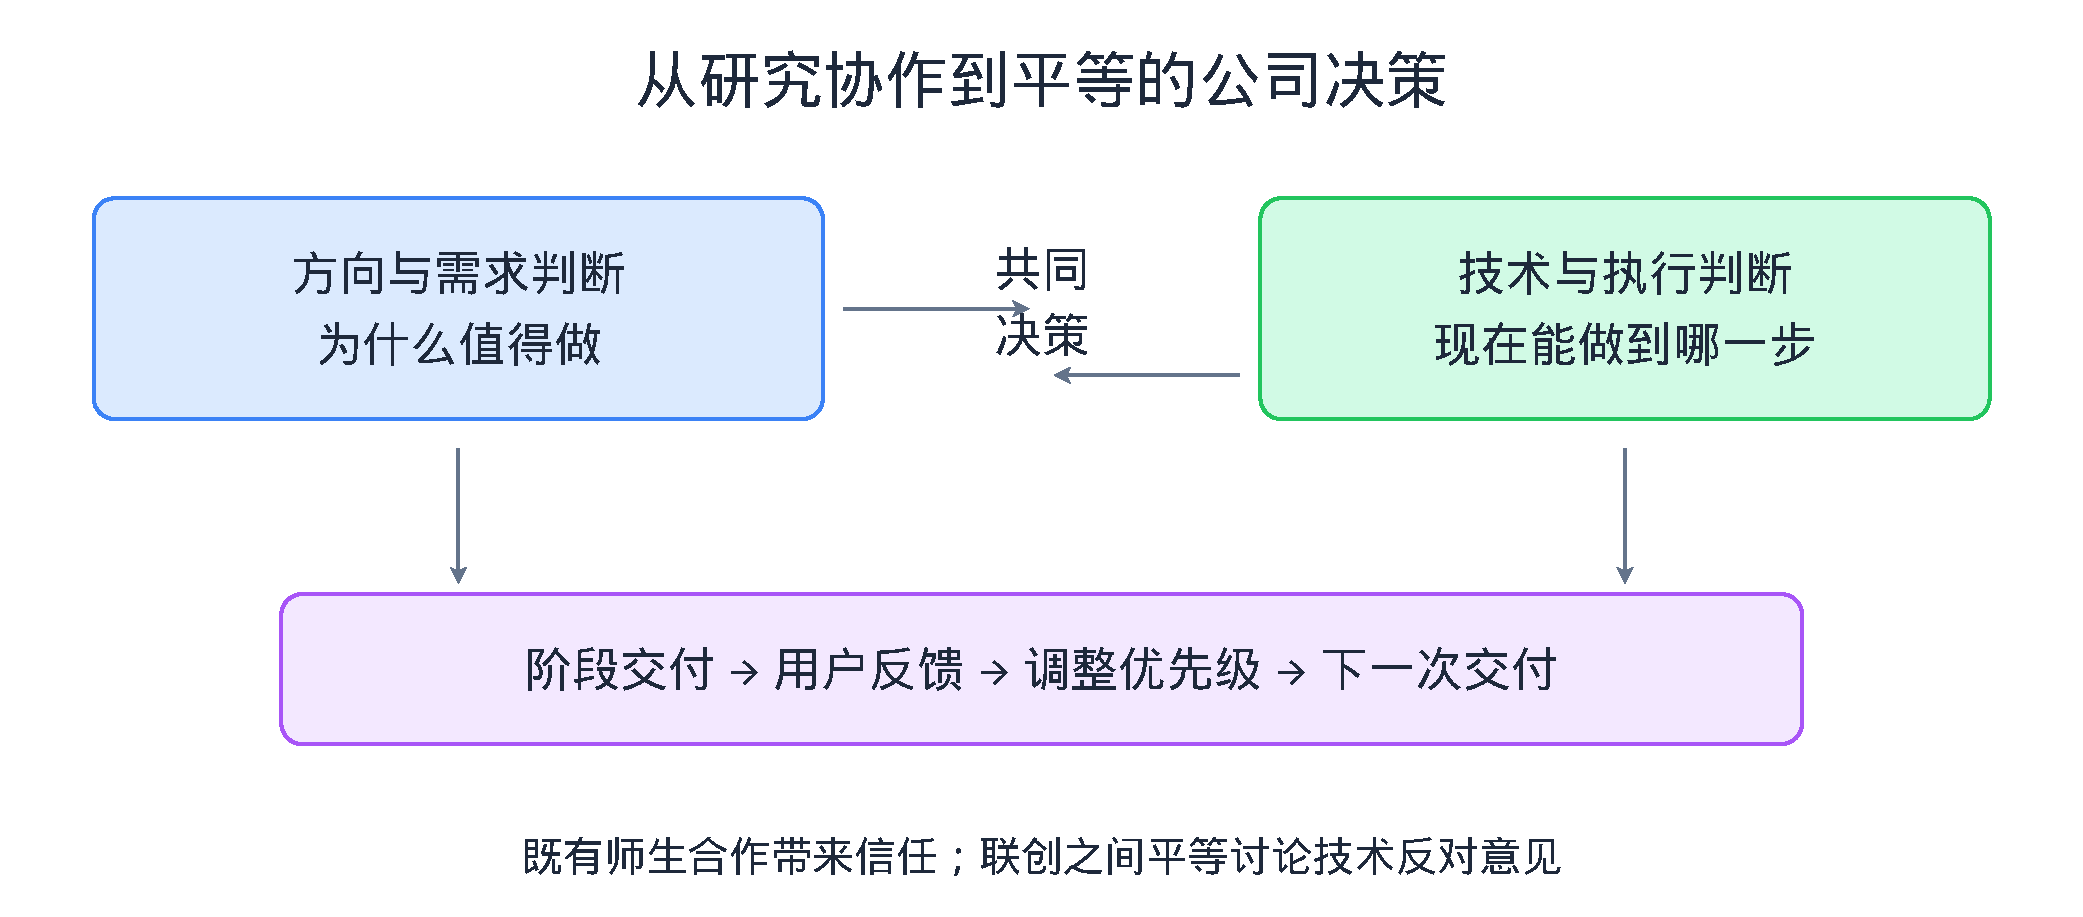
\includegraphics[width=\linewidth,height=.68\textheight,keepaspectratio]{assets/team-decisions.pdf}
\caption{从研究协作到平等的公司决策；依据节目口述整理（01:50:54–02:04:35）}
\end{figure}
\begin{knowledgebox}{读图：第六章 从开源研究组到有节奏的创业团队}
图上方左侧方框为“方向与需求判断：为什么值得做”，右侧方框为“技术与执行判断：现在能做到哪一步”；左右两框向中间发出相向的箭头，汇聚于中间的“共同决策”文字区域。同时，左右两框底部各有一条向下的箭头，共同指向下方的长框“阶段交付 \ensuremath{\rightarrow} 用户反馈 \ensuremath{\rightarrow} 调整优先级 \ensuremath{\rightarrow} 下一次交付”。图最底部总结道：“既有师生合作带来信任；联创之间平等讨论技术反对意见”。
\end{knowledgebox}
正是依靠这种方向互信、技术平等探讨并用真实用户反馈驱动迭代的团队机制，Tensormesh 得以在快速演进的 AI 基础设施生态中稳步推进；最后一章我们将把视野放到整个 AI 技术栈的接口演进与个人职业选择上。
\needspace{6\baselineskip}\subsection{本章小结}
\begin{enumerate}
\item 以公司化支撑基础设施的长期演进：面对核心博士生即将毕业的人员流动，以及将前沿研究成果持续转化为工业级基础设施的资源需求，江鋆晨团队选择与学生共同创立公司并引入风险投资，以建立全职工程与服务能力。
\item 补齐商业认知并与自己赛跑：学者创业不仅要从头学习路演（Pitch）与投资意向书（Term Sheet）谈判，还要在没有论文截稿日、早期尚无直接同业竞品的阶段保持紧迫感，通过内部节奏与阶段交付赶在大厂全面发力前筑牢壁垒。
\item 建立互信且平等的师生合伙关系：师生联创延续了长期合作积累的信任基础——学生信任导师的远景方向，导师信任学生的技术判断；而在公司决策中保持合伙人平等地位、尊重一线工程可行性的反对意见（Pushback），是团队良性运转的关键。
\end{enumerate}
\needspace{8\baselineskip}\section{第七章 接口、分离式架构与个人的下一步}
作为全篇的收官之章，本章从单个系统走向整个AI技术栈的演进规律与个人职业选择。我们将结合计算机网络的历史视角，理解OpenAI兼容接口为何能成为当前生态的“细腰”，探讨基础设施从整机集成走向分离式架构的潜力与工程前提，并梳理江鋆晨针对模型、基础设施与应用三个方向的分析，以及给不同年龄段学习者和从业者的具体建议。
\needspace{6\baselineskip}\subsection{OpenAI 兼容接口为什么像互联网的细腰}
在一个新兴技术生态高速生长的初期，各个层级的组件往往都在剧烈变动；但要让整个产业规模化运转，中间往往会有某些接口率先稳定下来，成为各方默认遵守的公共约定。在访谈中，江鋆晨从计算机网络研究者的视角出发，将当前广泛使用的OpenAI兼容接口（OpenAI-compatible API format）类比为互联网协议栈中的“细腰”（02:04:35–02:08:39）。

作为背景补充，计算机网络经典的“沙漏模型（Hourglass Model）”指的是：底层可以有各种不同的物理传输介质与链路技术，顶层可以有网页、视频、邮件等丰富的应用程序，而中间的网络层协议（Internet Protocol，简称 IP，负责在互联网络中寻址和路由数据包的协议）则像沙漏中间收窄的“细腰”一样，成为上下游共同承认的通信接口。因为有了稳定的细腰层，底层硬件和上层应用才能在降低直接耦合的情况下各自演进。与此同时，一旦某个中间层成为全行业广泛依赖的接口，想要在它上面做推翻式的改动就会面临很高的生态迁移成本。例如互联网早期的 IPv4（第四版互联网协议）沿用多年，后续设计的 IPv6（第六版互联网协议）虽然在地址空间和协议特性上做了诸多改进，且如今在全球范围内已获得广泛的实际部署，但从 IPv4 向 IPv6 的演进依然经历了长达二十余年的漫长过渡。

江鋆晨指出，今天大模型生态中稳定下来的这个接口，并不是指大家只能去调用 OpenAI 一家公司的服务，而是指 OpenAI API 兼容格式（OpenAI API compatible format，即一套通用的请求与响应数据格式约定）。如今，许多应用提供商、模型提供商和推理服务商都默认支持这套格式。当然，这种兼容格式属于生态中形成的接口惯例，不同于互联网里严格统一的底层网络协议，也不代表不同服务商的所有扩展功能都完全一致。但这一现象说明 AI 技术栈的某些层级正在快速形成行业共识；江鋆晨由此展望，随着跨服务复用与传输 KV 缓存的需求增多，KV 缓存数据层未来也有可能演化为生态中另一层相对稳定的公共接口。

\needspace{6\baselineskip}\subsection{分离式架构怎样增加选择}
除了软件接口的形成，硬件与系统架构的演进也可以从计算机历史中找到参照。当被问及 AI 基础设施领域还有哪些被低估的方向时，江鋆晨先顺带再次澄清了听众常问的一个概念混淆：大模型的 KV 缓存存的是注意力机制生成的两个浮点数张量，而不是传统数据库里的通用键值存储（Key-Value Store）。接着，他谈到了当前 AI 硬件生态中一个被他类比为“大型机化”的现象（02:08:39–02:12:16）。

按江鋆晨的观察，当前一些头部硬件提供商为了追求更高的利润空间（Margin）并提供整体打包的性能，倾向于把处理器、网络、存储等组件绑在一起，做成大型整机或机柜设备成套出售。他认为这种商业与工程打包方式，在思路上让人联想到 20 世纪 90 年代银行业等机构广泛采购的大型机（Mainframe）。回顾计算机发展史，当年大型机虽然性能强悍，但后来真正成为超大规模数据中心主流形态的，是通过分布式系统软件，把标准化、更具性价比的内存、存储、CPU 和网络连接并组合起来。

沿着这一历史类比，江鋆晨个人很看好分离式架构（Disaggregation，将原本紧耦合在一起的计算、内存、存储等资源拆分开，使其能够按需专门优化、灵活配置与替换的架构思路）在 AI 基础设施中的发展潜力。如果把分离式架构做到理想状态，系统中的各个模块可以针对特定任务专门设计并按需替换，而其中最核心的技术难点，则在于如何用高水平的系统软件把这些分离的模块高效组合起来。当然，在实际工程中，硬件模块的拆分与替换受制于网络带宽、跨节点延迟、全局调度以及接口协议兼容性等条件；江鋆晨也明确指出，这并不意味着头部大厂现有的集成式整机路线会消失，一体化大型设备依然会存在，但更灵活、更具延展性（Scalable）的分离式系统有望作为有力的竞争与补充方案成长起来。

\needspace{6\baselineskip}\subsection{模型、基础设施与应用的不同挑战}
面对快速演进的AI技术栈，现在的本科生与研究生在求职或规划研究方向时，究竟应该选择模型算法、基础设施（Infra），还是上层应用（Application）？江鋆晨针对这三个层级分别剖析了各自的核心挑战与能力要求（02:12:18–02:17:23）。

首先在模型层面，江鋆晨认为大模型本身仍有很大的发展空间，通用人工智能（AGI）也远未成为一个已经彻底解决的问题。对于读博做科研的学生来说，继续研究模型依然是个好方向，但建议不要去扎堆做大家已经反复做过的常规改良，而应该去探索真正新的模型结构或新路径。其次在应用层面，他坦言自己很难做出准确预测：一方面，AI 应用重塑传统商业模式的前景非常广阔；但另一方面，初创团队辛苦做出的某个应用功能，可能过一阵子就会被 Anthropic 或 OpenAI 等底层模型厂商的新一轮原生能力覆盖，这种演进态势充满了不确定性。

而对于选择 AI 基础设施方向的同学，江鋆晨建议去工业界历练，但他特别强调：不要去只做单纯写代码的工作。在 AI 编程能力快速提升的今天，单纯写程序的工作很容易被替代；AI 难以替代的是人的“担责能力”与“设计品味（Design Taste）”。他解释说，担责不是凭空拍胸脯保证代码不出问题，而是有能力把 AI 生成代码的过程纳入清晰的工程结构中——也就是具备设计品味，清楚地知道什么样的系统设计更持久、更好维护、更灵活。就像让 AI 画一幅画，如果创作者自己都分不清画得好不好，就很难把控质量；同理，如果基础设施工程师完全依赖 AI 生成设计，连自己写出的代码结构都无法判断和维护，就会失去核心价值。此外，在回顾个人过往选择时，他也重申了自己一贯的研究偏好：相比于偏居幕后、阶段性运行的训练基础设施（Training Infra），他个人更喜欢直面海量用户请求、处于台前且长期运行的推理基础设施（Inference Infra）。

\needspace{6\baselineskip}\subsection{按职业阶段选择有价值的学习环境}
在访谈的最后部分，江鋆晨针对处于不同年龄段和职业阶段的年轻人，分享了他个人的几点建议（02:17:25–02:25:19）。对于 22 岁即将本科毕业的大学生，他的建议是：“去做对自己最有挑战性的事情。”在他看来，22 岁时不必过早计较哪份工作眼下收入最高或最快能稳定下来，因为做对自己有挑战、难度高的事，往往能让人在年轻时学得最快。他回忆自己当年选择赴美读博，也是因为在本科时的他看来，能在网络顶会 SIGCOMM 上发表论文是一件极其困难的事，正是这种高难度挑战推动了他的成长。

对于二十六七岁正在攻读计算机博士（PhD）的学生，江鋆晨建议首先要明确自己未来是否真的想留在高校当老师。如果立志成为教授，那就必须在博士期间把所在细分方向做到顶尖；但如果不打算从事教职，就应该思考如何通过博士课题去接触工业界最前沿的真实问题。他解释说，如今的工业界与过去截然不同，企业里聚集了大量拥有博士或硕士背景的研究型人才——这并不是单纯因为工业界资金或算力资源多，而是因为人才密度的提升，使得工业界一旦看准某个值得研究的应用方向，推进速度会非常快。因此，不以教职为目标的博士生应当主动贴近工业界的技术最前沿（而不是去工业界做毫无技术深度的日常杂务）。同时，针对主持人在追问中提到的“既然如此是否可以干脆退学去工业界”，江鋆晨明确表示自己并没有建议学生退学，而且那些需要真正静下心来长周期探索的课题，依然是高校学术界不可替代的优势。

那么，对于二十五六岁已经在工业界工作、没有读博的年轻人，该如何应对原有工作内容可能被AI替代的危机感？江鋆晨指出了两条“充电”并建立个人差异化优势（Differentiator）的路径：一条路是在有一定经济积累后回到高校读博，实际上现在许多博士申请人正是来自工业界；另一条路则是加入初创公司（Startup）。因为初创公司面临着强烈的生存压力，每天都在逼着自己做出“别人无法替代的新东西”，在这样的环境里打拼同样是极高强度的充电。而到了30岁左右、处于职业生涯初期的阶段，人需要承担的现实责任变多了，不能再盲目鼓吹不计后果地冒险。江鋆晨认为，这个阶段如果能遇到志同道合的伙伴，在自身已有积累的基础上，一起去公司内部、学术界或创业赛道上做一件“有长期潜力但当时还没那么多人看好”的大事，会是非常珍贵的经历——正如他与几位实力出众的学生共同创业时，心中最大的责任感就是不要辜负和浪费年轻伙伴们本可以拿高薪的机会，大家携手把一件有价值的事真正做成。

\begin{knowledgebox}{沙漏模型与协议“细腰”的生态作用}
在计算机网络与系统设计中，“沙漏模型（Hourglass Model）”常用来解释复杂生态如何兼顾“底层多样性”与“上层丰富性”：
• 结构特征：系统分为多层，底层支持多种异构硬件或传输介质（沙漏下半部），顶层支撑多样化的应用场景（沙漏上半部），而中间层则收敛为少数共同遵守的通信接口或数据格式（沙漏的细腰）。
• 解耦作用：稳定的细腰接口降低了上下游之间的直接耦合，使上层应用与底层系统更容易通过适配公共接口来对接不同实现，而不必为每一种上下游组合单独重写整套逻辑。
• AI 生态类比：江鋆晨将当前广泛使用的 OpenAI API 兼容请求与响应格式比作 AI 生态早期形成的一处“细腰”惯例，并展望随着跨服务传输需求增加，KV 缓存管理也有望在基础设施内部沉淀出类似的稳定接口层。
\end{knowledgebox}
\begin{warningbox}{分离式架构（Disaggregation）需要克服哪些工程条件}
正文提到，与将处理器、网络、存储全部紧耦合打包出售的“整机/机柜式”方案相比，分离式架构试图将计算、内存、存储等资源拆分开，以获得更高的配置灵活性与性价比。要让这种模块化组合在 AI 推理生产环境中真正跑通，系统软件需要解决三个核心工程问题：
\begin{enumerate}
\item 高吞吐与低延迟传输：当 KV 缓存等大体积中间状态在分离的计算节点与存储池之间流动时，可结合压缩（如 CacheGen）、分块流式传输与高速互连来减少跨节点通信开销。
\item 跨层全局调度：调度器需要实时感知计算节点的显存水位与远端存储的缓存分布，决定何时将请求路由至已持有缓存的节点、何时跨网拉取缓存或直接重算。
\item 接口兼容与可维护性：不同厂商的芯片、推理引擎与存储介质需要通过标准化连接器对接，这也是为什么分离式系统最核心的壁垒在于“把分散模块聪明地组合起来”的系统软件能力。
\end{enumerate}
\end{warningbox}
\begin{table}[H]\centering\small
\caption{不同职业发展阶段的核心挑战与行动建议}
\begin{tabular}{>{\raggedright\arraybackslash}p{\dimexpr(\linewidth-6\tabcolsep)/3\relax}>{\raggedright\arraybackslash}p{\dimexpr(\linewidth-6\tabcolsep)/3\relax}>{\raggedright\arraybackslash}p{\dimexpr(\linewidth-6\tabcolsep)/3\relax}}
\toprule
所处阶段与群体 & 面临的核心处境或问题 & 江鋆晨建议的行动方向与机制\\\midrule
22岁即将毕业的本科生 & 容易过早追求工作稳定性、短期高薪或表面舒适的岗位 & 优先选择对自己最有挑战性的事情；在年轻阶段通过攻克高难度任务获得更快的能力成长\\[4pt]
26–27岁在读计算机博士（PhD） & 工业界聚集了大量高学历研究人才，前沿应用方向在企业的推进速度极快 & 先明确是否立志做教授；若不当老师，可研究与工业界最前沿紧密结合的课题，同时发挥学界长周期静心探索的优势\\[4pt]
25–26岁在工业界工作的工程师 & 日常重复性的常规编程工作面临被AI工具替代的风险，需要建立个人差异化优势 & 两条高强度“充电”路径：一是在有经济积累后回高校读博深造；二是加入有强烈生存意识的初创公司，参与构建不可替代的新产品\\[4pt]
30岁左右的职场初期从业者 & 个人与家庭责任增加，不适合盲目进行不计后果的单打独斗式冒险 & 兼顾现实责任与已有积累，寻找志同道合的伙伴，在企业内部、学术界或创业团队中共同投入有长期潜力但尚未被大众普遍看好的方向\\[4pt]
\bottomrule\end{tabular}\end{table}
借用计算机网络沙漏模型的历史视角，一个高速演进的技术生态往往会在中间沉淀出相对稳定的公共接口格式，从而让上下游模块在保持兼容的同时各自演进。下图展示了当前 AI 技术栈中的这一结构关系。
\begin{figure}[H]\centering
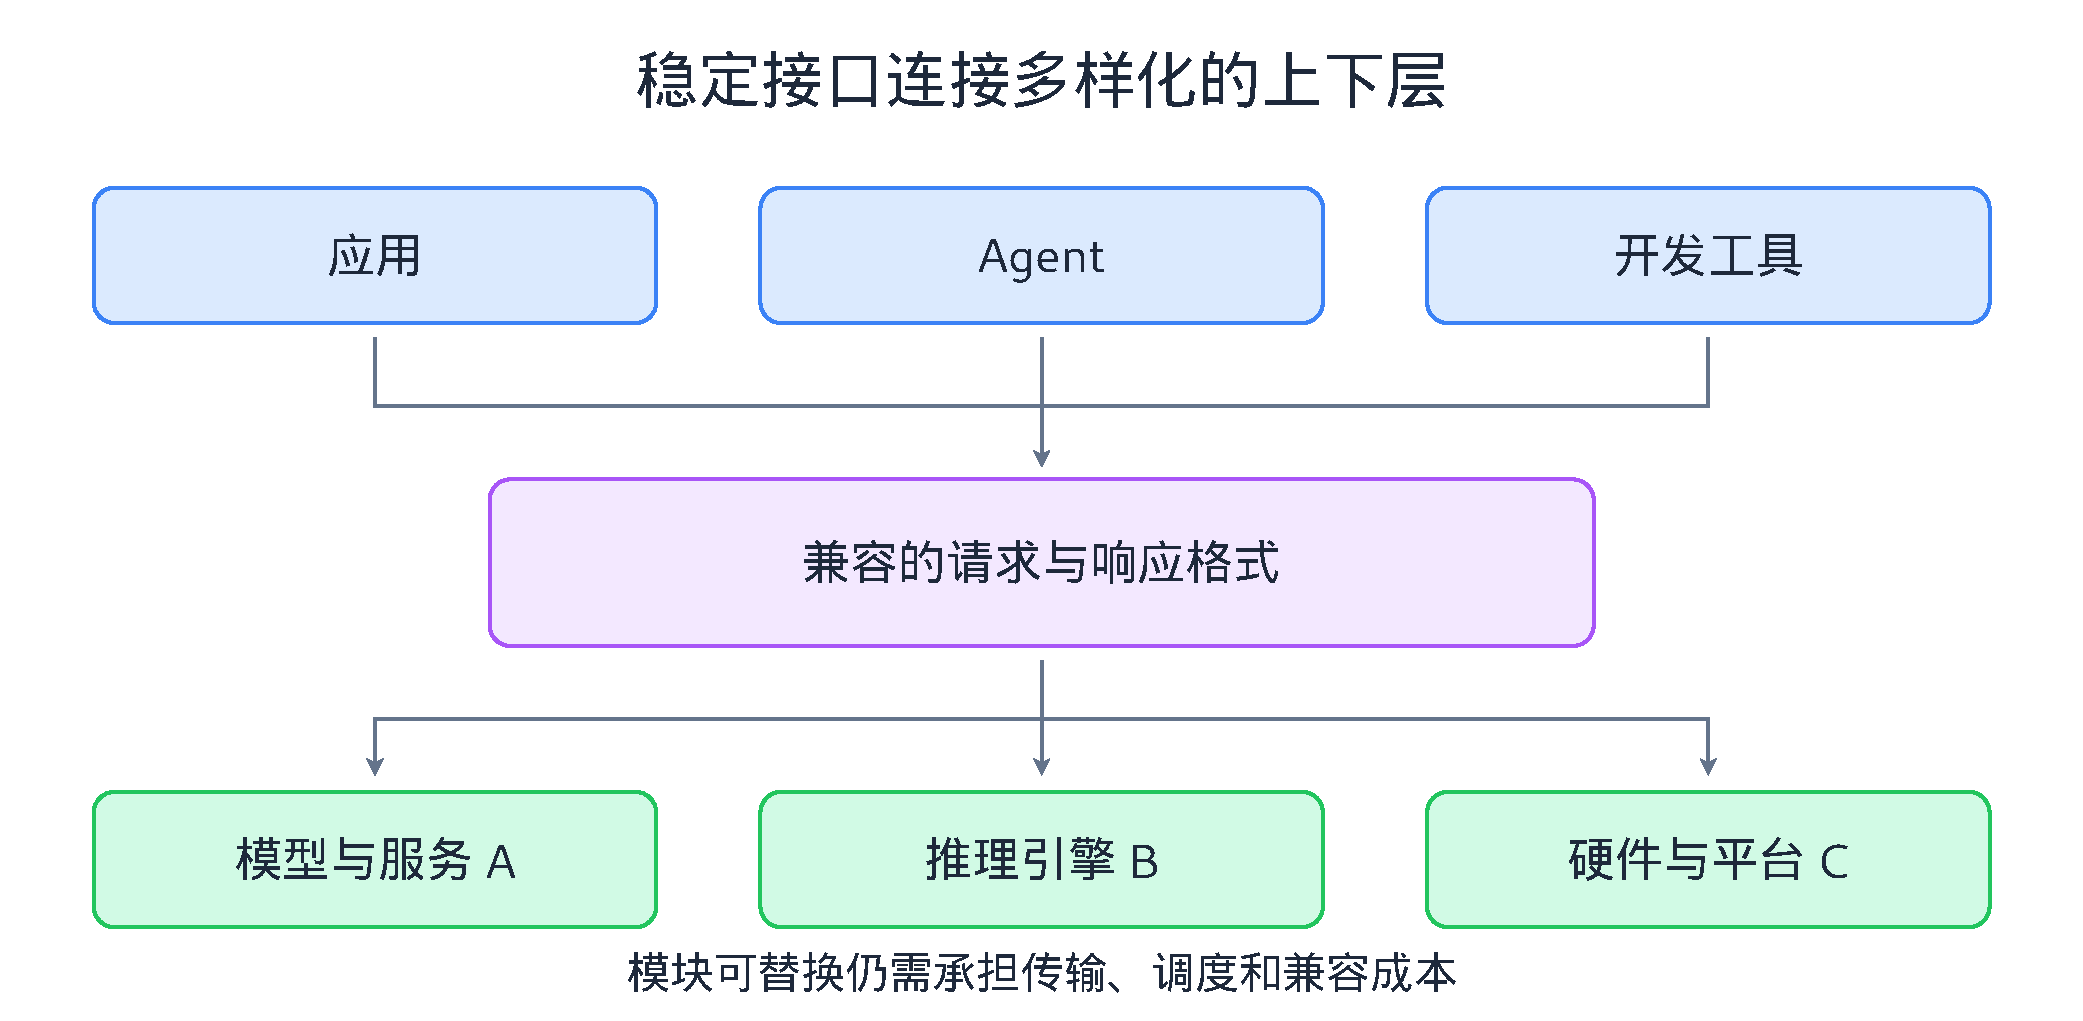
\includegraphics[width=\linewidth,height=.68\textheight,keepaspectratio]{assets/stable-interface.pdf}
\caption{稳定接口连接多样化的上下层；依据节目口述整理（02:04:35–02:12:16）}
\end{figure}
\begin{knowledgebox}{读图：第七章 接口、分离式架构与个人的下一步}
图上方并列三个方框：“应用”、“Agent”和“开发工具”，三者通过向下的折线箭头汇聚到中间的核心方框“兼容的请求与响应格式”。再从中间方框向下分出三条折线箭头，分别指向底部的三个方框：“模型与服务 A”、“推理引擎 B”以及“硬件与平台 C”。图最底部一行文字提醒了模块化背后的工程前提：“模块可替换仍需承担传输、调度和兼容成本”。
\end{knowledgebox}
理解了稳定接口与分离式架构在平衡生态扩展性与工程成本上的作用，年轻的学习者与工程师就能更清晰地看懂模型、基础设施与应用三层的技术走向，从而在各自的职业阶段做出更有定力的选择。
\needspace{6\baselineskip}\subsection{本章小结}
\begin{enumerate}
\item 稳定接口与分离式架构演进：OpenAI 兼容请求格式在当前 AI 生态中起到了类似互联网沙漏模型“细腰”的连接作用；而在硬件与系统层面，将计算、存储、网络按需组合的分离式架构，有望在系统软件克服通信与调度挑战后，成为紧耦合整机方案的重要竞争与补充形态。
\item 基础设施工程师的设计品味与担责：在 AI 辅助编程日益普及的背景下，AI 基础设施工程师的核心价值在于“设计品味（Design Taste）”与结构化担责能力——即判断何种系统架构更持久、更灵活、更易维护。
\item 分阶段的个人成长建议：22 岁可优先选择最有挑战的事以加速学习；在读博士生需明确是否有意任教，并主动接触工业界前沿研究问题；已工作的年轻工程师可通过读博或加入初创公司充电并建立差异化优势；到了 30 岁左右则需兼顾现实责任，寻找志同道合的伙伴共同投入有长期潜力的方向。
\end{enumerate}
\needspace{8\baselineskip}\section{总结与延伸}
回顾整场访谈，从 2010 年前后的视频流媒体到今天的大语言模型与智能体，江鋆晨从自己的研究经历中总结出一条线索：应用普及与高频交互会带来大量核心数据，专门负责传输、存储与共享的“数据层”因此有了发展空间。在大模型推理中，KV 缓存正是连接算力与存储的关键中间状态——它既是当下帮企业跳过重复 Prefill 计算、降低首字延迟与算力开销的工程手段，也承载着未来筛选、融合与优化模型运行期记忆的研究愿景。

如果你希望沿着本讲义的思路继续深入，可以按以下三条可操作的路径展开学习与实践：
\begin{enumerate}
\item 把经典系统论文当成“技术史”精读：挑选网络（如 CDN、HTTP 自适应流媒体）、大数据（如 HDFS、Spark）与大模型推理（如 vLLM、CacheGen、CacheBlend）各一至两篇代表作，对照阅读它们在各自时代面对了怎样的硬件与带宽突变，又抽象出了什么公共接口。
\item 动手测算并观察一次真实的 KV 缓存复用：利用本讲义第三章的字节估算公式，核算你常用开源模型在不同上下文长度下的显存占用；随后在本地或云端部署推理引擎与 LMCache，对比多轮长文档问答在开启跨请求缓存前后的首字延迟（TTFT）与存储传输开销。
\item 对照职业阶段锤炼“设计品味（Design Taste）”：无论你是即将毕业的学生还是在职工程师，在使用 AI 辅助编程时，有意识地把精力放在模块解耦、接口稳定性与系统可维护性的判断上；若有志于科研或创业，不妨深入工程一线寻找那些“工程师每天在争论、但尚未被写进论文”的真实瓶颈。
\end{enumerate}
\subsection{拓展阅读}
以下资料供回看节目、查阅术语与继续学习。
\begin{itemize}
\item 月球大叔：本期完整视频：\url{https://www.youtube.com/watch?v=yWTVEG9UIHo}
\item 官方完整逐字稿：\url{https://unclemoon.ai/blog/002-junchen-jiang/transcript/}
\item 官方访谈文章：\url{https://unclemoon.ai/blog/002-junchen-jiang/}
\item LMCache 官方项目：\url{https://github.com/LMCache/LMCache}
\item CacheGen：KV 缓存压缩与流式传输：\url{https://arxiv.org/abs/2310.07240}
\item CacheBlend：用于快速 RAG 的片段复用：\url{https://arxiv.org/abs/2405.16444}
\item Google IPv6 实际采用统计：\url{https://www.google.com/intl/en/ipv6/statistics.html}
\end{itemize}
\end{document}
